\documentclass[12pt]{ociamthesis}  % default square logo 
\usepackage[spanish]{babel} 
\usepackage[utf8]{inputenc}
\usepackage{float}% para el [H] haciendo que la imagen quede si o si donde se le ordeno

%\documentclass[12pt,beltcrest]{ociamthesis} % use old belt crest logo
%\documentclass[12pt,shieldcrest]{ociamthesis} % use older shield crest logo

%load any additional packages
\usepackage{amssymb}
\usepackage{listings}
\usepackage{xcolor}

%input macros (i.e. write your own macros file called mymacros.tex 
%and uncomment the next line)
%\include{mymacros}
\begin{document}

%this baselineskip gives sufficient line spacing for an examiner to easily
%markup the thesis with comments
\baselineskip=18pt plus1pt


%set the number of sectioning levels that get number and appear in the contents
\setcounter{secnumdepth}{3}
\setcounter{tocdepth}{2}

\definecolor{dkgreen}{rgb}{0,0.6,0}
\definecolor{dred}{rgb}{0.545,0,0}
\definecolor{dblue}{rgb}{0,0,0.545}
\definecolor{lgrey}{rgb}{0.9,0.9,0.9}
\definecolor{gray}{rgb}{0.4,0.4,0.4}
\definecolor{darkblue}{rgb}{0.0,0.0,0.6}

\lstdefinelanguage{cpp}{
	backgroundcolor=\color{lgrey},  
	basicstyle=\footnotesize \ttfamily \color{black} \bfseries,   
	breakatwhitespace=false,       
	breaklines=true,               
	captionpos=b,                   
	commentstyle=\color{dkgreen},   
	deletekeywords={...},          
	escapeinside={\%*}{*)},                  
	frame=single,                  
	language=C++,                
	keywordstyle=\color{purple},  
	morekeywords={BRIEFDescriptorConfig,string,TiXmlNode,DetectorDescriptorConfigContainer,istringstream,cerr,exit}, 
	identifierstyle=\color{black},
	stringstyle=\color{blue},      
	numbers=right,                 
	numbersep=5pt,                  
	numberstyle=\tiny\color{black}, 
	rulecolor=\color{black},        
	showspaces=false,               
	showstringspaces=false,        
	showtabs=false,                
	stepnumber=1,                   
	tabsize=5,                     
	title=\lstname,                 
}


%\maketitle                  % create a title page from the preamble info
\begin{titlepage}
	\begin{center}
		
\includegraphics[width=5cm]{logo2.png}\\
		\vspace{1cm}
		FACULTAD DE INGENIERÍA\\
		INGENIERÍA CIVIL INFORMÁTICA\\
		\vspace{1cm}
		\LARGE{\textbf{Una arquitectura caché para redes ICN basada en comportamiento de usuario} \\}
		\vspace{1cm}
		\small{Tesis para optar al grado de ingeniero civil en informática.}\\
		\vspace{2cm}
		\textbf{Autor:} \\
		Mathias Nicolas Velilla Brandau.\\
		\vspace{1cm}
		\textbf{Profesores guía:} \\
		Carlos Gomez-Pantoja\\
		Miguel Gutierrez\\
		\vspace{1cm}
		Santiago de Chile, Chile.\\
		\vspace{1cm}
		Junio, 2017
	\end{center}
\end{titlepage}


\begin{romanpages}          % start roman page numbering
\tableofcontents            % generate and include a table of contents
\listoffigures              % generate and include a list of figures
\listoftables % indice de tablas
\end{romanpages}            % end roman page numbering

\chapter{Introducción}
\section{Motivación}

El nacimiento del Internet en el año 1958 en EE.UU. a través de ARPA (\textit{Advanced Researchs Proyects Agency}) tuvo como objetivo la comunicación entre diversas entidades con propósitos investigativos. La aparición de la conmutación por paquetes implementadas en los mecanismos de comunicación sentó las bases para el desarrollo de esta nueva tecnología, la cual hoy en día ha revolucionado la informática y las comunicaciones como ninguna otra cosa convirtiéndose en una herramienta de índole mundial. Un mecanismo el cual nos permite diseminar información de manera inmediata, generando un medio de colaboración e interacción entre las personas y los ordenadores, desconociendo su ubicación física.\\

Durante los años 2000 - 2008 el uso diario del Internet en las personas americanas rondaba entre un 60\% y 70\% \cite{mossberger2007digital}. Este crecimiento en el uso de la Internet, conlleva también a un aumento de la información presente en la web, dando como resultado el desarrollo de aplicaciones las cuales deben interactuar con un gran numero de usuarios y analizar una sobresaliente cantidad de información. Por este motivo Internet ha sido impulsado por demandas de aplicaciones cada vez más emergentes y capacidades de las nuevas redes de comunicación, ha convertirse en un mosaico arquitectónico que resulta en una creciente complejidad y vulnerabilidades imprescindibles, entregando violaciones de capas, proliferación de subcapas, y la erosión del modelo de extremo a extremo. Es bajo esta eventualidad que todos los cambios efectuados concluyen en un aumento de la complejidad, lo cual se traduce en una Internet osificada. Es por esta razón que los problemas anteriormente señalados no se encuentran directamente relacionados con los protocolos o mecanismo específicos del Internet actual. Más bien son causados esencialmente por la incapacidad de integrar nuevos mecanismos. Esto quiere decir que los problemas son causados por la arquitectura de Internet y podrían ser resueltos con un nuevo diseño de arquitectura de Internet \cite{muller2009future}.\\

La creciente demanda de una distribución altamente escalable y eficiente del contenido ha motivado el desarrollo de futuras arquitecturas de Internet basadas en objetos de datos nombrados (NDO, por sus siglas en inglés), por ejemplo, páginas web, videos, documentos u otras informaciones. El enfoque de estas arquitecturas se conoce comúnmente como redes centradas en información (ICN). Por el contrario, las redes actuales se centran en el \textit{host}, donde la comunicación se basa en \textit{hosts} nombrados, por ejemplo, servidores web, PC, portátiles, teléfonos móviles y otros dispositivos \cite{ahlgren2012survey}.\\

Las arquitecturas ICN aprovechan el almacenamiento en red para el almacenamiento en \textit{caché}, la comunicación multilateral a través de la replicación y los modelos de interacción que desacoplan a los remitentes y receptores. El objetivo común es lograr una distribución eficiente y confiable de los contenidos en donde cada uno de estos es nombrado única e independientemente desde la ubicación del productor (servidor), facilitando el almacenamiento en \textit{caché} en los nodos intermediarios. Así, por ejemplo, los consumidores solicitarán contenidos enviando el denominado paquete de interés, el cual lleva el nombre del contenido, mientras que el productor o cualquier nodo que mantenga una copia del contenido puede responder a la petición realizada \cite{ahlgren2012survey}.\\

A su vez, los usuarios ya antes mencionados como consumidores, realizan peticiones en la web, las cuales siguen una conducta dinámica caracterizándose por un elevado sesgo entre los diferentes conjuntos de peticiones. En otras palabras, dentro del universo de peticiones generadas existen conjuntos de peticiones que son regularmente solicitadas por los consumidores en intervalos de tiempos distintos, por lo contrario, otras peticiones escasamente son solicitadas. Dicho lo anterior, también existen situaciones dentro de un intervalo acotado de tiempo, donde surgen explosivamente peticiones las que se caracterizan por poseer un contenido en común, las cuales nacen por el desarrollo de un evento de interés popular teniendo como resultado un aumento sustancial en la demanda generada a los nodos, teniendo como consecuencia latencia y congestión en las redes.


\section{Desafíos}
Los desafíos que trae consigo llevar a cabo el proyecto de titulo, son los de aprender a investigar, comprender nuevos conceptos, realizar una ingeniera inversa de como funciona el simulador y la de plantear una nueva arquitectura \textit{caché} que ayude a mejorar la eficiencia del \textit{caché} y consigo la red.

\section{Contribución de la tesis}
El aporte entregado por el proyecto de título, se puede identificar inicialmente por la creación y diseño de una nueva arquitectura de memoria \textit{caché} para los nodos de las redes \textit{ICN} (\textit{Information Centric Network}), considerando el comportamiento de los usuarios por medio del tráfico de red. En segundo lugar, se debe incorporar una estrategia de \textit{caché} (políticas de admisión, desalojo y reemplazo) y que será implementada en un simulador denominado \textit{SIM} (\textit{Named Data Networking Simulator}), todo esto con el fin de mejorar resultados de eficiencia de la memoria \textit{caché} (\textit{Hit's, Miss}) en comparación con otras arquitecturas \textit{caché} que se encuentran por defecto dentro del simulador (LFU, FIFO). No obstante, a continuación se detallarán las contribuciones efectuadas por este trabajo:\\
\begin{itemize}
	\item Diseño de una nueva arquitectura \textit{caché} bajo el paradigma de las redes ICN, que contenga una subdivisión de tres grupos capaces de retener diferentes tipos de peticiones (intereses) de modo que la eficiencia del nodo se vea afectada positivamente. En cuanto a la división de la memoria \textit{caché}, el primer segmento se encarga del almacenamiento de peticiones del tipo ráfaga, la segunda de guardar las de tipo permanente y para la última sección, la recaudación de peticiones de tipo variable.\\
	\item Creación de una topología de redes ICN, utilizando el simulador ndnSIM, la cual contenga dentro de sus nodos la arquitectura \textit{caché} anteriormente señalada con la finalidad de inyectar trafico de datos en base al comportamiento usuario para la obtención de resultados empíricos respecto a la nueva arquitectura \textit{caché} diseñada.\\
\end{itemize}


\section{Estructura de la tesis}
A continuación se realizará una breve reseña de cómo se estructura el siguiente trabajo.\\

El capítulo 2 abarca la descripción del problema, en el se define el objetivo general, específicos, hipótesis y los alcances que contiene el proyecto de título, incluyendo también la descripción de la metodología de trabajo utilizada para el progreso del trabajo.\\

El capítulo 3 posee el marco teórico, en el cual se definen diferentes conceptos esenciales para el entendimiento del proyecto del título. Dicho lo anterior se encuentran los siguiente conceptos: Redes centradas en la información (ICN), ndnSIM, aplicaciones web de gran escala, el \textit{caché}, estructura y políticas de reemplazo del \textit{caché} existentes, finalizando con el comportamiento del usuario de manera donde se explica la ley de Zipf y se detallan los tipos de peticiones de usuario.\\

En el capítulo 4 se presenta una revisión bibliográfica de los trabajos realizados respecto a las arquitecturas \textit{caché} y las políticas de \textit{caché} implementadas en redes ICN, además del revisión de trabajos dentro del simulador ndnSIM, todo esto con el fin de diseñar una arquitectura de \textit{caché} que no exista en la literatura.\\

\chapter{Descripción del problema}
\section{Contextualización}
NDN es una arquitectura de red basada en contenido perteneciente al paradigma ICN, que tiene como objetivo desplazar la actual arquitectura del Internet. Logrando así aumentar diversidad de contenido en red, reducir la congestión en red, tiempos de respuesta y carga del servidor.\\

Para hacer lo anteriormente señalado la arquitectura de red NDN consta de nodos intermediarios que poseen memoria \textit{caché}. Las que guardan entradas que están ligadas a una respuesta pre-computada, que fueron realizadas por las peticiones de los usuarios. Así cuando una nueva petición de un usuario sea enviada, si el nodo contiene en su memoria \textit{caché} la respuesta pre-computada de la petición esta sera devuelta al usuario.\\

Como la memoria \textit{caché} tiene limite de capacidad esta cuenta con algoritmos denominados políticas, los que permiten mantener actualizada su información y por ende generar mayor cantidad de \textit{hit's}, lo que se traduce en un mejor rendimiento de \textit{caché}. También la memoria \textit{caché} posee múltiples esquemas que permiten un mejor funcionamiento de esta. Por otro lado las peticiones realizadas por los usuarios en el Internet poseen patrones de comportamiento que varían en el tiempo y en su frecuencia. Alguno de estos patrones son: Ráfagas, Permanentes, Periódicas.\\

El proyecto de título tiene como objetivo proponer una arquitectura \textit{caché} considerando el comportamiento del usuario, para los nodos de la arquitectura de red NDN  y implementarlo en el simulador de red NDNSIM. La arquitectura constara de asignar un espacio del \textit{caché} la cual se dividirá en tres secciones de consultas (ráfaga, permanente y dinámicas).\\

El resultado de la solución propuesta, sera contrastada con estrategias que vienen por defecto en el simulador NDNSIM y nombradas en el estado del arte del este trabajo. Analizando así la tasa de \textit{hit} de los experimentos realizados y verificando la eficacia de la arquitectura \textit{caché} propuesta.\\

\section{El problema}

\subsection{Declaración del problema}
La cantidad de información presente en la red del Internet es de proporciones inimaginables. Información que es almacenada en servidores y solicitada por los usuarios en forma de consultas y de manera constante, para luego ser procesada y satisfacer la respuesta del usuario. Para reducir la carga del servidor producida por la búsqueda de la respuesta en \textit{back-end}, se propone la utilización de una red basada en contenidos, específicamente la arquitectura de red NDNSIM, la cual contiene una interconexión de nodos caché.\\

El \textit{caché} tiene un almacenamiento limitado, es por eso que es importante mantenerlo actualizado respecto a las consultas de los usuarios, para así tener una mayor tasa de \textit{hit's} y reflejada en una menor carga del servidor. Para lograr esto, es que se utilizan esquemas de \textit{caché} y también las llamadas políticas de admisión, reemplazo y eliminación las cuales ayudan a mantener el almacenamiento caché actualizado.\\

En los trabajos mencionados en la sección 4, específicamente el trabajo \cite{tarnoi2014performance} en donde exponen una modificación tanto del esquema del \textit{caché} y a las políticas de reemplazo, con el fin de mejorar las métricas propuestas. O bien trabajos como el de \cite{mun2017cache} en el cual desarrollan nuevos paquetes.\\

También se tiene que tener en consideración que las consultas de los usuarios arrastran un patrón de comportamiento que varia según el tiempo y su frecuencia. Comportamiento que provoca congestión en red(Cuello de botella), sobre carga de servidores, aumento en tiempo de respuesta, disminución de la eficiencia del \textit{caché}, fallas en nodos, etc.\\

\subsection{Diagrama de Ishikawa}
En la Fig.\ref{diagrama_ishikawa} se muestra el diagrama de Ishikawa con el fin de
comprender los problemas relacionados con la ineficiencia del \textit{caché}.

\begin{figure}[!htb]
	\centering
	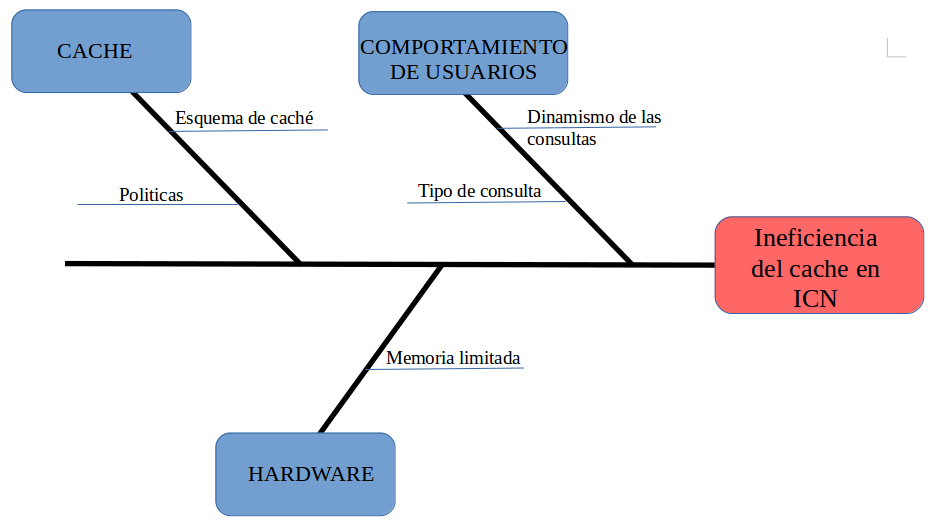
\includegraphics[width=12cm]{Imagenes/Diagrama_ishikawa}\\
	\caption{Diagrama de Ishikawa. Fuente: Elaboración propia.}
	\label{diagrama_ishikawa}
\end{figure}
\section{Objetivos}
\subsection{Objetivo general}
Optimizar la eficiencia del \textit{caché} en una arquitectura NDN por medio del diseño de una arquitectura \textit{caché} basada en comportamiento de usuario.
\subsection{Objetivos específicos}
Para lograr el objetivo general de la tesis se requiere cumplir con los siguientes objetivos específicos.
\begin{itemize}
	\item Analizar patrones de comportamiento.
	\item Proponer una solución \textit{caché} para una red basada en contenido con una arquitectura NDN.
	\item Realizar una evaluación experimental .
\end{itemize}


\subsection{Alcance de los objetivos}

El proyecto de título se limita a la propuesta y experimentación de una arquitectura \textit{caché} para la red basada en contenido NDN. Donde se utilizará un  paquete ndnSIM de código abierto, que implementa la pila de protocolos NDN para el simulador de red NS-3, para ejecutar simulaciones.\\

Este trabajo se enfoca principalmente en el \textit{caché} y en  utilizar las políticas tanto de reemplazo, admisión y eliminación (LFU, LRU, RR, FIFO). Las cuales serán implementadas en cada sección de \textit{caché} según corresponda al comportamiento de usuario. Definiendo parámetros de entrada y una topología especifica. Con el fin de obtener resultados respecto a la tasa de \textit{hit}. Por eso como trabajo futuro queda analizar como afecta el comportamiento del borde de la red, en la arquitectura \textit{caché} propuesta.

\begin{table}[H]
	
	\begin{tabular}{|p{3cm}|p{3cm}|p{3cm}|p{3cm}|p{2cm}|}
		\hline
		\textbf{Situación actual} & \textbf{Objetivo específico} & \textbf{Resultado esperado} & \textbf{Métrica} & \textbf{Criterio de éxito}\\ \hline
		Comportamiento dinámico y variable en el tiempo de las consultas de los usuarios. & Analizar patrones de comportamiento. & Conjuntos de trabajos que señalen los distintos tipos de patrones de comportamiento. & Número de patrones definidos ($P_n$) & $P_n$ $\geq$ 3\\ \hline
		
		Variados trabajos que buscan mejorar la eficiencia del \textit{caché} algunos de ellos presentados en el estado del arte. & Proponer una solución \textit{caché} para una red basada en contenido con una arquitectura NDN. & Esquema o política \textit{caché}. & Numero patrones usados en la solución ($SP_n$) & $SP_n \geq 2$\\ \hline
		
		Esquemas y políticas \textit{caché} (Admisión y reemplazo) ya presentes en el simulador (LFU,,FIFO, RR). & Realizar una evaluación experimental de la solución \textit{caché} propuesta. & Gráficos con resultados obtenidos. & Tasa de \textit{hit's}($T_h$) Numero contexto($N_c$) &  $T_h \geq 5\%$ ; $N_c \geq 2$. \\ \hline
		
	\end{tabular}
	\caption{Alineamiento de objetivos}
	\label{Tabla_alineamiento}
\end{table}

\chapter{Marco teórico}

\section{Information Centric Networking}
ICN (\textit{Information-Centric Networking}) es un paradigma que pretende motivar la transición arquitectónica de la actual arquitectura centrada en el \textit{host} a centrada en la información, para difundir de manera eficiente y flexible la enorme información generada por una variedad de aplicaciones. En esta dirección de investigación, se han propuesto muchos enfoques durante los últimos años, de los cuales para el desarrollo de este trabajo se centrara en NDN.(Figura 3.1)\hfill

	\begin{figure}[!htb]
		\centering
		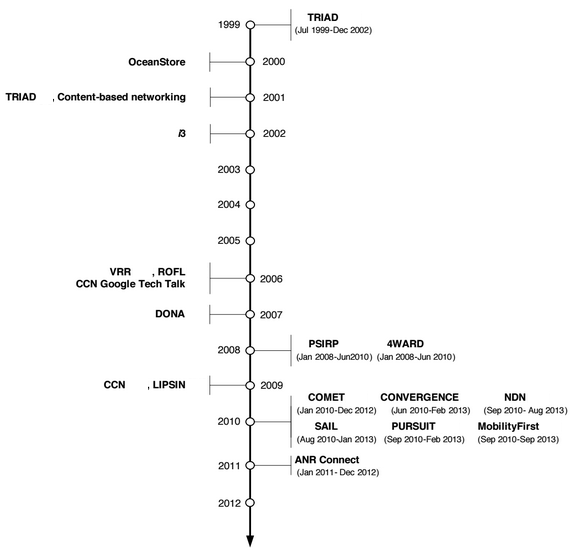
\includegraphics[width=10.3cm]{Imagenes/Linea_Temporal_ICN_limpia.png}\\
		\caption{Cronología de los principales hitos de ICN \cite{xylomenos2014survey}.}
		\label{fig:mesh1}
	\end{figure}
	
\textit{Named Data Networking} (NDN) es una de las arquitecturas futuras para el Internet, con años de investigación sobre el uso de la red y de los problemas no resueltos en arquitecturas contemporáneas del Internet como IP \cite{nsf10528}\cite{nsf13538}. La arquitectura NDN tiene su origen en el proyecto \textit{Content-Centric Networking} (CCN) que Van Jacobson divulgo por primera vez en el año 2006 en una charla tecnológica de Google \cite{jacobson2006new}.\\

El proyecto NDN financiado por EE.UU desarrolla aun más la arquitectura CCN anteriormente mencionada, reconfigurando la pila de protocolos del Internet intercambiando la cintura delgada de la arquitectura de Internet por el de datos nombrados, empleando diversas tecnologías de red por debajo de la cintura para la conectividad, incluyendo IP. También, NDN con el fin de optimizar el uso de recursos, contiene una capa de estrategia media que se ubica entre la capa de datos nombrada y las tecnologías de red, mientras que una capa de seguridad lleva a cabo las funcionalidades de seguridad directamente a los datos nombrados \cite{xylomenos2014survey}(Fig. \ref{Arq_reloj_arena}).\\

	\begin{figure}[!htb]
		\centering
		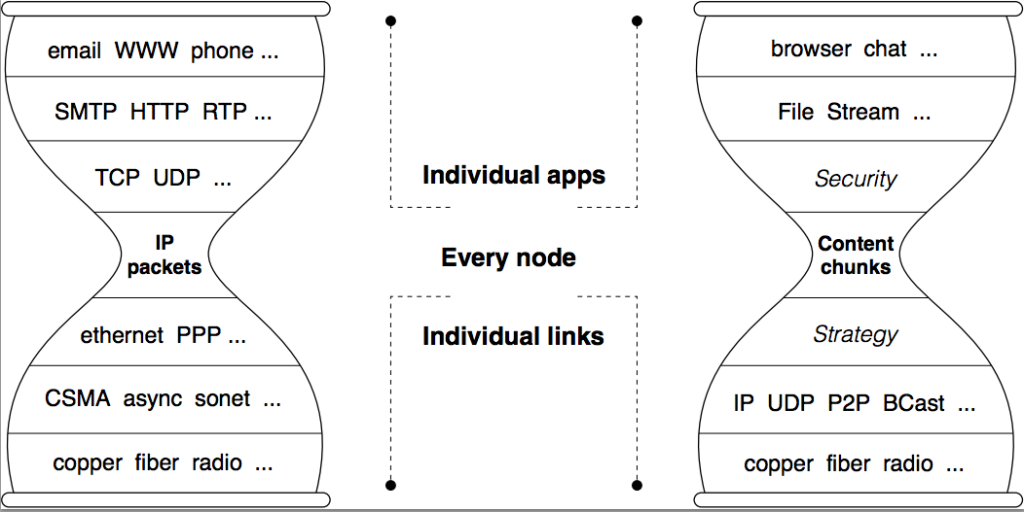
\includegraphics[width=12cm]{Imagenes/Protocolo_IP_vs_NDN.png}\\
		\caption{Arquitecturas de reloj de arena de Internet y NDN \cite{named_data_networking}.}
		\label{Arq_reloj_arena}
	\end{figure}

Dicho lo anterior, la principal abstracción de ICN es el NDO (\textit{Named Data Objects}), la que se define como la unidad de datos direccionales que se encuentra dentro de una red centrada en la información, siendo capaces de representar una colección de bytes o una información en específico. Así mismo cada uno de los objetos de datos existentes posee un nombre vinculado a el, logrando verse como fragmentos de datos nombrados sin semántica alguna y caracterizándose por su granularidad la cual varía desde el tamaño del paquete hasta los objetos completos \cite{kutscher2016information}\cite{ahlgren2012survey}.\\

Los objetos de datos con nombre se desligan de la ubicación, la aplicación, el almacenamiento y los medios de transporte, dando paso al almacenamiento en \textit{caché} y un bajo costo y ubicua replicación en la red, esperando como resultado una mayor eficiencia y seguridad, una mayor escalabilidad respecto a la demanda de información/ancho de banda y una superior robustez en escenarios de comunicación desafiantes \cite{kutscher2016information}.\\

La arquitectura NDN se compone de dos tipos de NDO, los paquetes de interés (\textit{Interest Packet}) y los paquetes de datos (\textit{Data Packet}), presentes(Fig. \ref{Paquetes_NDN}), siendo el nombre de estos de tipo jerárquico, similares a una URL, como por ejemplo /aueb.gr/ai/main.html. Los cuales son enviados por dos tipos de usuarios: el primero denominado consumidor, entidad encargada de enviar una solicitud de un NDO a la red (\textit{Interest}), y por otra parte un productor, que es la entidad encargada publicar NDO's en la red, los cuales serán solicitados por un consumidor y enviados (\textit{Data}).\\

\begin{figure}[!htb]
		\centering
		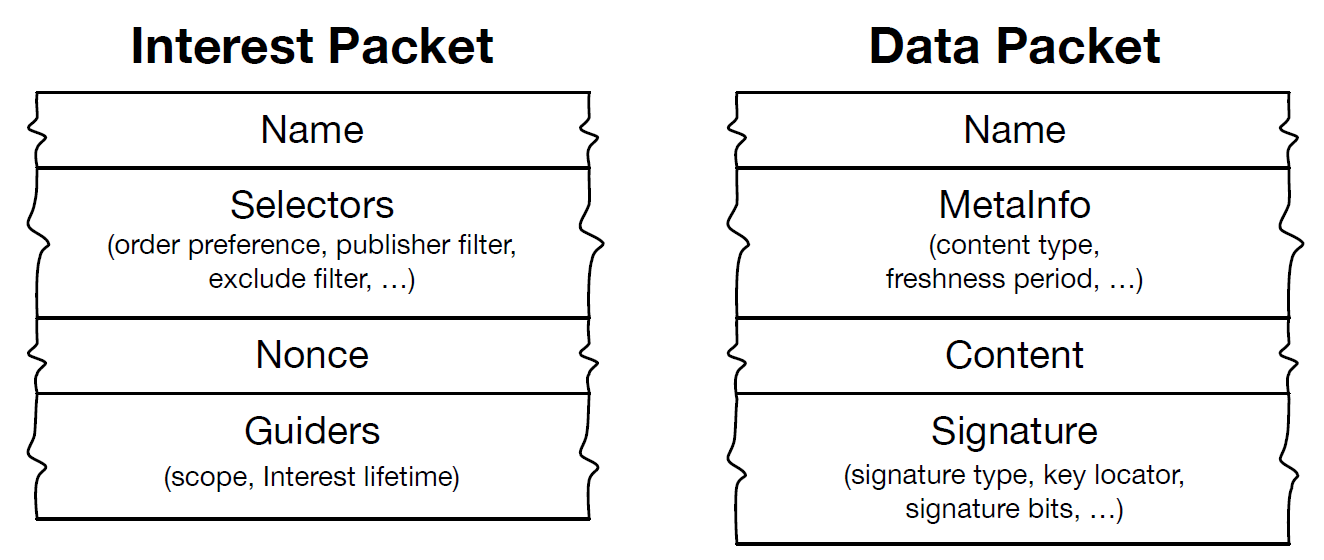
\includegraphics[width=10cm]{Paquetes_NDN.png}\\
		\caption{Paquetes NDN.}
		\label{Paquetes_NDN}
\end{figure}
 
Adicionalmente esta arquitectura también cuenta con nodos intermediarios entre los consumidores y los productores denominados CR (\textit{Content Routers}), los cuales le entregan a la red un aumento en la replicación de información y consigo una mayor resolución de consultas. Los nodos contienen tres estructuras de datos principales (Fig. \ref{Arquitectura_ndn}):

\begin{itemize}
	\item\textbf{\textit{Forwarding Information Base} (FIB):} El FIB se utiliza para reenviar paquetes de interés hacia fuentes potenciales de datos coincidentes. Es casi idéntico a un IP FIB, excepto que permite una lista de interfaces salientes en lugar de una sola. Esto refleja el hecho de que CCN no está restringido a reenvío en un árbol de expansión. Permite múltiples fuentes de datos y puede consultarlas todas en paralelo \cite{jacobson2009networking}.\\
	\item \textbf{Almacén de contenido (\textit{Content Store}, CS):} El almacenamiento en \textit{caché} de los NDO es una parte integral del servicio ICN. Todos los nodos potencialmente tienen \textit{cachés}, incluyendo nodos en redes de infraestructura de ejecución de operadores y redes domésticas dirigidas por usuarios, así como terminales móviles. Las solicitudes de NDO pueden ser satisfechas por cualquier nodo que contenga una copia en su \textit{caché}. ICN combina así el almacenamiento en \textit{caché} en el borde de la red, como en P2P y otras redes de superposición, con almacenamiento en \textit{caché} en la red (por ejemplo, \textit{cachés} de web transparentes). El almacenamiento en \textit{caché} es genérico, es decir, es independiente de la aplicación y se aplica a todos los proveedores de contenido, incluido el contenido generado por el usuario \cite{jacobson2009networking}.\\
	\item \textbf{\textit{Pending Interest Table} (PIT):} El PIT realiza un seguimiento de los Intereses enviados hacia arriba hacia la(s) fuente(es) de contenido de forma que los datos devueltos puedan ser enviados aguas abajo a su(s) solicitante(s) \cite{jacobson2009networking}.\\
\end{itemize}

	\begin{figure}[!htb]
		\centering
		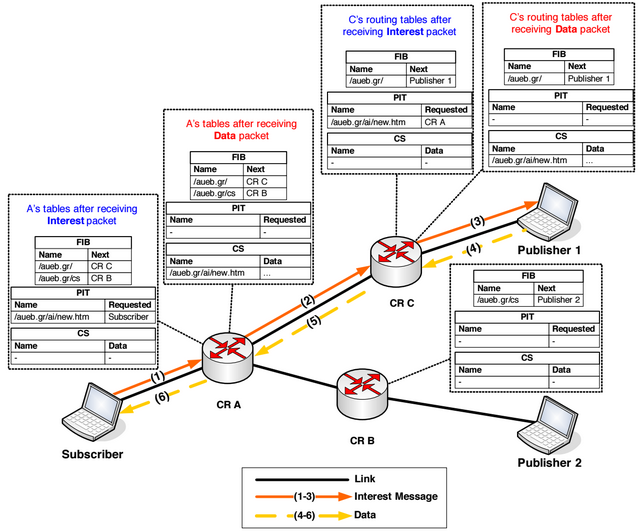
\includegraphics[width=10cm]{Nodo2.png}\\
		\caption{Arquitectura NDN, CR significa Content Router, FIB para Forwarding Information Base, PIT para Pending Interest Table y CS para Content Store. Fuente: A Survey of Information-Centric Networking Research \cite{xylomenos2014survey}.}
		\label{Arquitectura_ndn}
	\end{figure}


\section{Caché}
La cantidad de usuarios van en aumento día a día, por lo que las aplicaciones web con un gran número de usuarios tienen que ser capaces de soportar grandes volúmenes de consultas y transacciones de datos (millones), las cuales poseen una patrón de comportamiento definido, este tema se abordará en la sección 3.3. Una de las tecnologías que existe para apaciguar el acceso incesante a información de los servidores, es la de un lugar de almacenamiento destinado a archivar las consultas y su respuesta pre-computada, denominado \textit{caché}.\\

El \textit{caché} es una de las partes más importante dentro de los servicios web y motores de búsqueda \cite{altingovde2009cost},\cite{aggarwal1999caching}. Principalmente el \textit{caché} es un espacio de almacenamiento (memoria) de acceso rápido, en donde se retienen las consultas más reiteradas hechas por los usuarios y sus respuestas, entregando una gran cantidad de ventajas entre las que se encuentran:

\begin{itemize}
	
	\item Reducir la latencia de acceso a los documentos, esto se debe a que los objetos que son accedidos con mayor frecuencia se encuentran almacenados en un nodo de \textit{caché} cercano, lo que disminuye el tráfico en la red, permitiendo que los objetos que no están en \textit{caché} puedan también ser recuperados con mayor rapidez \cite{wang1999survey}.
	
	\item Reducir el consumo de ancho de banda, lo que permite disminuir la congestión y el tráfico en la red \cite{wang1999survey}.
	
	\item Reducir la carga de trabajo en los servidores web \cite{wang1999survey}.
	
\end{itemize}

Siendo las características deseables para una arquitectura \textit{caché} las siguientes: robustez (capaz de no generar fallos o bloquearse), acceso rápido (disminuir latencia), eficiente, escalable, estable, adaptable y simple de implementar \cite{wang1999survey}. Por ello una de las finalidades más importantes en el \textit{caché} es la de obtener el mayor número respecto a la tasa de \textit{hit}, en otras palabras, conseguir que una gran parte de las consultas realizadas por el usuario, que ingresan al \textit{caché} cuente con una respuesta pre-computada.\\

En la arquitectura NDN, el \textit{caché} de los CR juega un rol importante al momento de satisfacer las peticiones del usuario (consumidor). A modo de que sin la presencia del \textit{caché}, el paradigma de las redes ICN no sería válida, causando así que los productores (servidores), procesen un volumen elevado de consultas simultáneas. La importancia del \textit{caché} en la arquitectura NDN de las redes ICN radica en que esta requiere de una difuminación eficiente de la gran cantidad de consultas realizadas diariamente por lo usuarios, de manera que sean respondidas de forma rápida.\\

El \textit{caché} es limitado, por lo que al completar su capacidad máxima es necesaria la  implementación de algoritmos que permitan el control del almacenamiento. Estos algoritmos son las denominadas políticas, de las cuales existen tanto de admisión, reemplazo y desalojo. Dada la gran cantidad de consultas que generan los usuarios en el Internet es que se hace necesaria la creación de nuevas políticas que permitan una mejor eficiencia del \textit{caché}.\\



\subsection{Organización del Cache}

En la arquitectura NDN el \textit{caché} (\textit{Content Store}) se encuentra presente en los distintos nodos (CR) incluyendo también a los consumidores y productores. Donde la entrada que posee un CS es una tupla $<$Name, Data$>$ siendo \textit{Name} el NDO \textit{Interest} y \textit{Data} el NDO que responde dicho \textit{Interest}. Como se señaló en el punto anterior, el almacenamiento en \textit{caché} es limitado, por lo que la entrada de tuplas deben ser constantemente variadas, dando la posibilidad del ingreso de nuevas entradas, las cuales tienen mayor probabilidad de aumentar la tasa de \textit{hit} en \textit{caché}. A continuación se definirán las políticas ya señaladas. 

\subsubsection{Política Admisión}
Esta política es la encargada del administrar la entrada a la memoria \textit{caché}, a través del bloqueo de entradas que no sean constantemente requeridas en el futuro, a raíz de que lo anterior producirá un aumento en la tasa de miss del \textit{caché} \cite{baeza2007admission}, disminuyendo la eficiencia del nodo CR.\\

Esto ocurre cuando la memoria en \textit{caché} se encuentra en su máxima capacidad, por lo que no es posible almacenar una nueva entrada, motivo por el cual se pone en marcha la política de desalojo respectiva para descartar una entrada del \textit{caché} y ingresar la nueva entrada. Pero debido a que la nueva entrada puede generar escasos \textit{hit's}, entonces se deben de llevar a cabo las políticas de admisión las cuales tomarán la decisión de si la nueva entrada es guardada en la memoria \textit{caché} o bien se mantendrá la entrada propuesta para el desalojo de \textit{caché}.\\

\subsubsection{Política Desalojo o Reemplazo}
Las política de desalojo o reemplazo se llevan a cabo cuando la memoria \textit{caché} se encuentra llena, por lo que es necesario liberar espacio para dar oportunidad a otras entradas entrantes, principalmente la idea es descartar una entrada la cual posee una baja probabilidad de lograr ser un \textit{hit} en \textit{caché} \cite{baeza2007admission}.\\

Los objetos web, los NDO en el caso de la arquitectura NDN contienen diferentes variables que son tomadas en cuenta para decidir si salen o se quedan en \textit{caché}, como lo son el tiempo de la última referencia, el tamaño, tiempo de expiración y el tiempo desde su última modificación.\\

Algunas de políticas de desalojo conocidas dentro de la literatura, son \textit{Least Frequently Used} (LFU) y \textit{Least Recentently Used}
(LRU) \cite{gomez2014servicios}\cite{gan2009improved}\cite{cambazoglu2010refreshing}. Dentro del simulador ndnSIM se encontraran las ya anteriormente señalados algoritmos de reemplazo, además del algoritmo FIFO, y un cantidad no menor de variaciones de los algoritmos señalados, con su respectiva variable que permitirá decidir que entrada seleccionar.\\

\subsubsection{Eliminación de entradas antiguas}
Principalmente la política de eliminación de entradas antiguas son las encargadas de mantener el almacenamiento en memoria \textit{caché} actualizado.

\subsection{Estructura del caché}
Anteriormente se vio que es posible caracterizar el \textit{caché} según las políticas que utiliza este mismo, pero también es factible agrupar el \textit{caché} en dos categorías: Estático y dinámico.

\subsubsection{Caché Estático}
Tal como dice su nombre, son \textit{cachés} que no cuentan con variabilidad de contenido durante un intervalo de tiempo amplio, estos tipos de \textit{caché} se basan generalmente en información acumulada históricamente y es actualizada a largo plazo.\\

Dentro del contexto de los motores de búsqueda, el \textit{caché} estático aglomera en memoria las entradas más habituales, por medio del análisis de registros históricos de las entradas efectuada por los usuarios. Siendo algunas de las características a tomar en cuenta para ser incorporada en el \textit{caché}: la cantidad de usuarios que realizaron la misma consulta, la frecuencia de la consulta, proporción de clics hechos por los usuarios a las URL que entregaron como respuesta a la consulta, además de la estabilidad temporal de la frecuencia de una consulta.

Realizada una vez la captación de las entradas más habituales, serán guardadas en \textit{caché} y actualizada oportunamente.\\

\subsubsection{Caché Dinámico}
Son \textit{cachés} en donde el contenido varía constantemente, por lo tanto se trata de incorporar dentro del \textit{caché} las entradas que tienen alta probabilidad de ser solicitadas en un futuro. Por lo tanto al ser una \textit{caché} que varía en el tiempo, el contenido almacenado debe ser frecuentemente actualizado, por medio de políticas de desalojo o reemplazo. Inicialmente este tipo de \textit{caché} esta vacía, para luego ir llenándose periódicamente a medida que se ingresan entradas en \textit{caché} (tuplas) hasta llenarse y luego implementar las políticas de reemplazo para mantenerse actualizado.

\subsection{Arquitectura de caché}

\subsubsection{Arquitectura de caché jerárquico}
Son \textit{cachés} que se asimilan a la estructura de un árbol, sus nodos \textit{caché} se clasifican en padre e hijo. El \textit{caché} padre no se comunica con sus hijo, pero el hijo si puede solicitar al padre. En esta arquitectura \textit{caché} se sitúan nodos \textit{caché} en múltiples niveles de red \cite{rodriguez2001analysis}. Esta arquitectura consta de cuatro niveles: inferior, institucional, regional y nacional. Los cuales van siendo recorridos en el orden respectivo a medida que la peticiones no son solucionadas por estas mismas. Si la petición no es solucionada por ningún nivel de \textit{caché} entonces se redirecciona al servidor original para encontrar el documento solicitado, para luego insertar esta el documento solicitado en el nivel más bajo de la jerarquía y dejando copias en los nodos intermedios. De modo que si continúan las solicitudes de ese documento, esta seguirá escalando a lo alto de la jerarquía. En la Fig. \ref{topologia_cache_jerarq} se observa la topología del \textit{caché} jerárquico.

\begin{figure}[!htb]
	\centering
	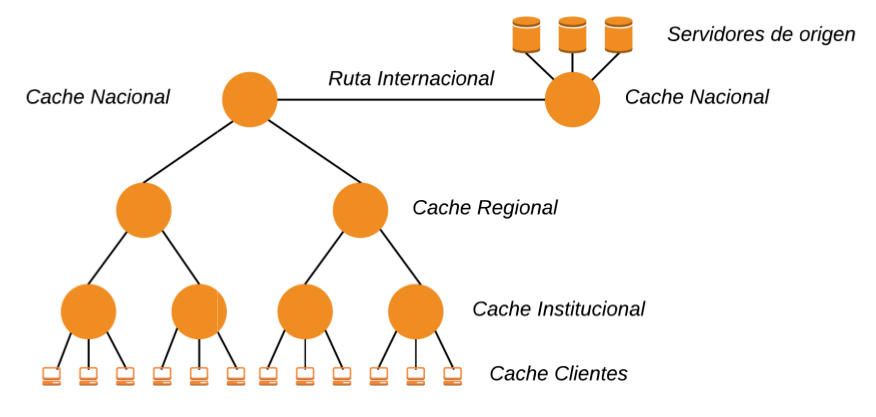
\includegraphics[width=12cm]{Imagenes/Topologia_cache_jerarquico}\\
	\caption{Topología de \textit{caché} jerárquico. Fuente: Arquitectura para la distribución de documentos en un sistema distribuido a gran escala \cite{sosa2002arquitectura}.}
	\label{topologia_cache_jerarq}
\end{figure}
 
\subsubsection{Arquitectura de caché distribuido}
A diferencia del \textit{caché} anteriormente señalado, el \textit{caché} distribuido, solo cuenta con un nivel de jerarquía, el \textit{caché} institucional. En donde sus nodos se encuentran conectados entre si para así ir a buscar el documentos a otros nodos que lo puedan contener, en caso de generarse un \textit{miss} en la búsqueda de alguno de estos(Ver Fig. ). A continuación se describirán algunas ventajas del \textit{caché} distribuido en contraste con el \textit{caché} jerárquico según \cite{nagaraj2004web}: menor uso de espacio en disco, mayor balance de carga y tolerancia a fallos.

\begin{figure}[!htb]
	\centering
	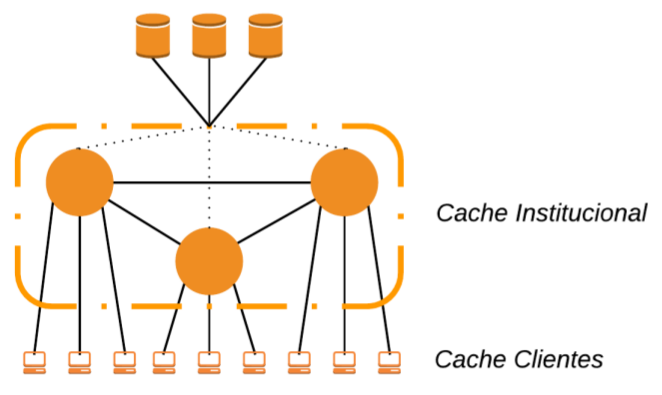
\includegraphics[width=9cm]{Imagenes/Topologia_cache_distribuido}\\
	\caption{Topología de \textit{caché} distribuido. Fuente: Arquitectura para la distribución de documentos en un sistema distribuido a gran escala \cite{sosa2002arquitectura}.}
	\label{topologia_cache_distribuido}
\end{figure}

\subsubsection{Arquitectura de caché híbrida}
Los \textit{caché} híbridos son una combinación del \textit{caché} jerárquico y el \textit{caché} distribuido. Los nodos \textit{caché} pueden cooperar con otros \textit{cachés} que se encuentren en el mismo nivel de jerarquía o en un nivel superior a través del \textit{caché} distribuido. En la Fig. \ref{topologia_cache_hibrido} se observa la topología que puede seguir una arquitectura de \textit{caché} híbrido.

\begin{figure}[!htb]
	\centering
	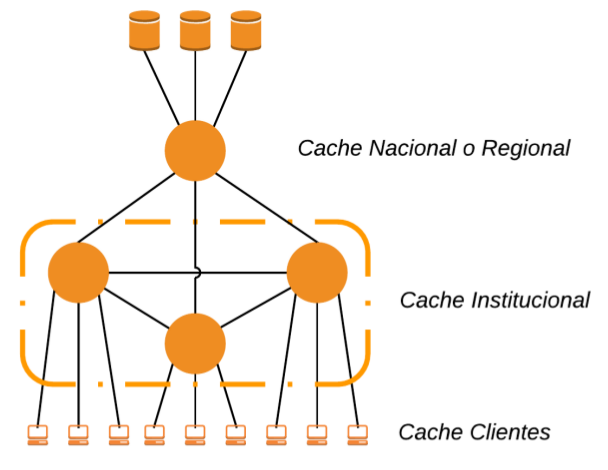
\includegraphics[width=9cm]{Imagenes/Topologia_cache_hibrida}\\
	\caption{Topología de \textit{caché} híbrida. Fuente: Arquitectura para la distribución de documentos en un sistema distribuido a gran escala \cite{sosa2002arquitectura}.}
	\label{topologia_cache_hibrido}
\end{figure}

\pagebreak
\section{Comportamiento de usuario}

El comportamiento de usuario se puede definir como, un área que intenta encontrar características, patrones o conductas de los usuarios en algún contexto específico, como por ejemplo en las redes sociales, en algunos sistemas de compras, y otras. Esto es de importancia para las empresas en general, ya que pueden mejorar sus ofertas de productos o hacer sistemas más eficientes que consideren alguna conducta repetitiva de los usuarios.

\subsection{Ley de Zipf}
La llamada ley de Zipf, formulada en la década de 1940 por George Kingsley Zipf \cite{zipf2013psycho}\cite{zipf2016human} es una ley empírica la cual establece que una cantidad menor de palabras son altamente utilizadas, mientras que existe un conjunto mayoritario de palabras que son raramente usadas. El comportamiento o bien patrón que tienen estas palabras siguen la fórmula:\\
\begin{equation}
\frac{1}{n}
\end{equation}\\

Donde \textit{n} corresponde a la \textit{n}-ésima palabra ordenada por frecuencia decreciente. El comportamiento anteriormente señalado no solo ha sido estudiado para las palabras, también ha sido analizado en el contexto de los motores de búsqueda, específicamente al comportamiento de las consultas, obteniendo como resultado que estas también siguen una distribución ``zipfianas" \cite{baeza2012modeling}\cite{cambazoglu2010refreshing}\cite{gan2009improved}\cite{lempel2003predictive}\cite{wang2013impact}\cite{saraiva2001rank}\cite{xie2002locality}.



\subsection{Peticiones de usuarios}
Los usuarios del Internet de ahora ya no son los mismos usuarios del Internet de años atrás, la información que necesitaban los primeros usuarios, ya no es la misma información que necesitan los usuarios de ahora y al igual que la moda, esta va variando en el tiempo. De la misma manera, las consultas generadas por los usuarios va cambiando en el tiempo, en función de distintas circunstancias que afectan el interés de los usuarios a la hora de realizar consultas, como lo son la economía, el deporte, desastres naturales, fechas importantes, temporada, eventos sociales y/o culturales, etc.\\

Teniendo en cuenta lo anterior y la frecuencia con la que se lleva a cabo cierto tipo de consulta, es que sera logrado encontrar patrones de conducta los cuales permiten clasificar los distintos tipos de consultas. Entre las clasificaciones de consultas más conocidas se encuentran las consultas periódicas, las consultas en ráfaga y las consultas permanentes, las que serán detalladas a continuación.

\subsubsection{Consultas Periódicas}
Corresponden a consultas que poseen un aumento en su frecuencia en un intervalo definido de tiempo, para luego disminuir hasta llegar a su frecuencia constante, todo esto de manera periódica (meses, semanas, días, horas, años, etc.). Dicha información permite anticipar la sobrecarga de los servidores, sin tener la necesidad de utilizar un algoritmo que permita la admisión en \textit{caché}. A continuación en la figura se muestra un ejemplo de una consulta de tipo periódica, correspondiente a la consulta ``18 de septiembre''\\

\begin{figure}[!htb]
	\centering
	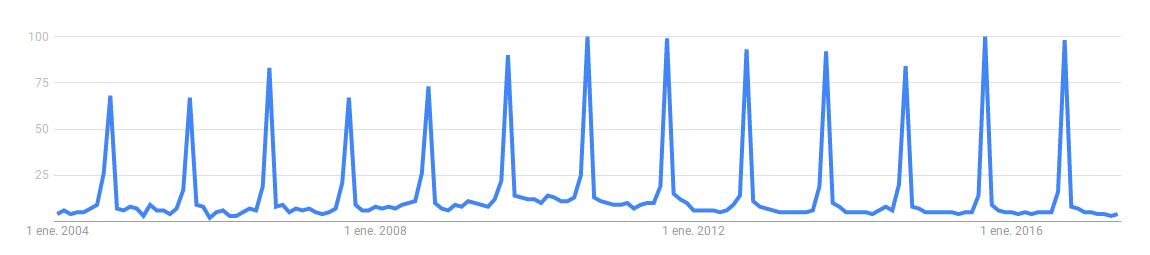
\includegraphics[width=15cm]{18_sept_google_trend.png}\\
	\caption{Frecuencia de consulta periódica: ``18 de Septiembre'' (2004-2016). Fuente: Google Trends.}
	\label{fig:mesh1}
\end{figure}

\subsubsection{Consultas Ráfagas}
Este tipo de consultas se caracteriza principalmente por poseer una frecuencia constante en el tiempo, la cual se ve afectada por un evento en específico, ya sea de índole social, económico, cultural, etc, llamando así el interés de los usuarios en general. Esto provoca que la frecuencia respecto a un tema en específico aumente bruscamente hasta alcanzar un \textit{peack}, para luego ir reduciéndose a medida que pasa el tiempo, como consecuencia del desinterés que comienzan a tener los usuarios respecto al tema mencionado. Un ejemplo de este tipo de consultas corresponde a la ``muerte de Fidel Castro" tal como se muestra en la Figura \ref{google_trend_muerte_Fidel_Cast}.\\

\begin{figure}[!htb]
	\centering
	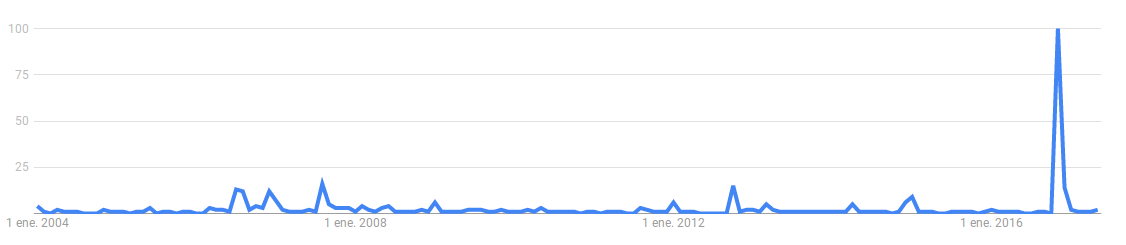
\includegraphics[width=15cm]{muerte_fidel_castro.png}\\
	\caption{Frecuencia de consulta ráfaga: "Muerte de Fidel Castro"(2004-2017). Fuente: Google Trends.}
	\label{google_trend_muerte_Fidel_Cast}
\end{figure}

Además, las consultas en ráfaga no solo afectan a una consulta en específico, si no que también a todo conjunto de consultas que tengan algún tipo de relación con el evento en particular que llevó al alza en este tópico. En la Figura \ref{google_trend_histo_Fidel_Cas} se observa como también la consulta ``Historia de Fidel Castro" posee un patrón ráfaga de la misma forma que la consulta ``muerte de Fidel Castro" y durante los mismos intervalos de tiempo.\\

\begin{figure}[!htb]
	\centering
	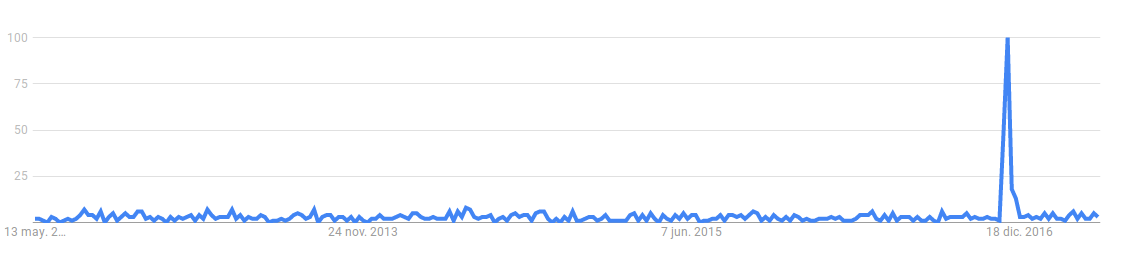
\includegraphics[width=15cm]{historia_Fidel_Castro.png}\\
	\caption{Frecuencia de consulta rafaga: ``Historia de Fidel Castro" (2012-2017). Fuente: Google Trends.}
	\label{google_trend_histo_Fidel_Cas}
\end{figure}

Uno de los problemas más serios que producen estas consultas debido al aumento en el volumen de consultas solicitadas, es la generación de desbalance en los nodos con respuestas pre-computadas en \textit{caché}, como también una congestión al acceso de la información en los servidores.\\
\clearpage

\subsubsection{Consultas Permanentes}
Finalmente las consultas permanentes, son definidas como aquellas que poseen una continuidad en la frecuencia que son solicitadas en intervalos largo de tiempo. En simples palabras, son consultas en que el paso del tiempo no afecta abruptamente su frecuencia. En la Figura \ref{google_trend_google} se adjunta una consulta del tipo permanente la cual corresponde a ``YouTube".\\

\begin{figure}[!htb]
	\centering
	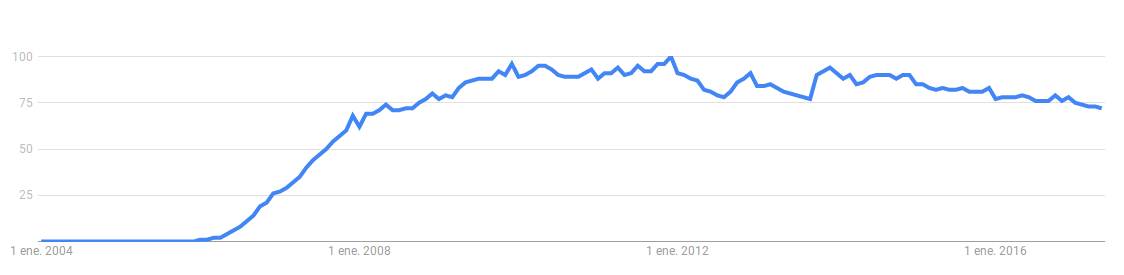
\includegraphics[width=15cm]{YouTube.png}\\
	\caption{Frecuencia de consulta permanente: ``YouTube" (2004-2017). Fuente: Google Trends.}
	\label{google_trend_google}
\end{figure}

Bajo este contexto, muchos son los trabajos encontrados en la literatura \cite{zhang2013two}, \cite{markatos2001caching}, \cite{ozcan2012five}, \cite{kumar2008new}, los cuales tienen como conclusión que destinar un espacio estático en \textit{caché} para guardar las consultas permanentes, lo que permite aumentar el rendimiento del \textit{caché}, mejorando la tasa \textit{hit} de este mismo. Cabe recordar que las consultas permanente se obtienen de registros históricos, los cuales son analizados para determinar cuales son consultas permanente y cuales no, tomando en cuenta su frecuencia. \\ 


%*******************************************************
\chapter{Estado del arte}
\section{NDNSIM}
\subsection{On Performance of Cache Policies in Named Data Networking \cite{ran2013performance}}

En \cite{ran2013performance} se propone el diseño de una política de reemplazo de \textit{caché} basada en la popularidad del contenido (CCP), la cual tiene en cuenta el factor de popularidad y una nueva estructura de datos denominada "Tabla de popularidad de contenido (CPT) sobre la base de retención del \textit{Content Store} (CS), \textit{Pending Interest Table} (PIT) y la \textit{Forwarding Interest Base} (FIB). Con el fin de beneficiar las métricas de golpe de \textit{caché}, carga del servidor y el promedio de rendimiento de la red en comparación con las políticas de \textit{caché} LFU y LRU ya presentes en el simulador.\\

Para que esto sea posible, según \cite{ran2013performance} las estrategias \textit{caché} deben poseer dinamismo en cuanto al contenido almacenado en \textit{caché}, siguiendo los dos siguientes puntos:

\begin{itemize}
	\item Ser capaz de adaptarse a los cambios rápidos en el modo de transmisión dinámica de red.
	\item No puede ser afectado por el contenido de la alternativa temporal.
\end{itemize}

De modo que las demandas anteriormente señaladas son saciadas por la política de reemplazo de \textit{caché} basada de popularidad (CPP) propuesta.\pagebreak

\subsubsection{Calculo de la popularidad de un contenido}

CCP añade una nueva estructura de datos CPT, la cual contiene toda la información sobre la popularidad del contenido almacenada en CS, incluyendo el nombre del contenido, el \textit{hit} en \textit{caché}, la popularidad anterior y actual. Dicha estructura de datos sa va actualizando cada vez que termina un ciclo de conteo, obteniendo así el \textit{ranking} actual de popularidad del contenido por medio del \textit{hit} de \textit{caché} y la popularidad anterior.
A continuación se describe la formula de calculo para la popularidad del contenido:

\begin{equation}
P[i+1] = \frac{N[i]*\alpha+P[i]}{\alpha+1}
\end{equation}

\begin{equation}
\alpha=1+c*T
\end{equation}

En donde P[i] corresponde a la popularidad del contenido en \textit{caché} y N[i] los \textit{hit's} del contenido en \textit{caché} en el momento del conteo actual. En cuanto a $\alpha$ ($\alpha>1$) es el coeficiente de peso de la popularidad del contenido, T el ciclo de conteo y C el coeficiente proporcional de $\alpha$ y T. Señalado lo anterior, para este trabajo desarrollado se considero que c = 0,5 y T = 8.\\

Pero para calcular la popularidad de un contenido, no solo se toma en cuenta el peso entre la popularidad anterior y actual, si no que también se considera la influencia de la ultima red \textit{hot pot}. Logrando así por medio de la expansión de 4.1 la obtención de 4.3.

\begin{equation}
P[i+1] = \frac{N[i]*\alpha+P[i]}{\alpha+1}
	   = \frac{N[i]*\alpha}{\alpha+1} + \frac{N[i-1]*\alpha}{(\alpha+1)^2} + \frac{N[i-2]*\alpha}{(\alpha+1)^3} + ...
\end{equation}

Llegando así a la conclusión de que con el tiempo, el numero de \textit{hit's} anterior posee una influencia menor en la popularidad de l contenido, lo que refleja de mejor manera la popularidad del contenido en la red actual. Obteniendo resultados como los del siguiente ejemplo, pudiéndose ver que el segundo contenido tiene una popularidad anterior mucho mayor que la primera pero con un menor \textit{caché} actual.

\begin{figure}[!htb]
	\centering
	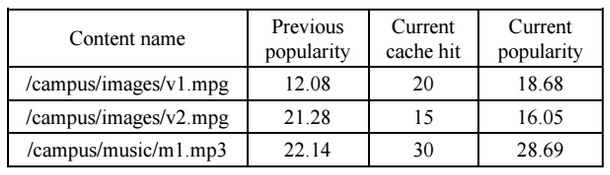
\includegraphics[width=10cm]{Imagenes/Paper1.1/TablaPopularidadContenido}\\
	\caption{Tabla de popularidad de contenido. Fuente: On Performance of Cache Policies in Named Data Networking \cite{ran2013performance}}
	\label{tabla_popularidad_contenido}
\end{figure}

\pagebreak

\subsubsection{Estrategia de reemplazo}

La estrategia de reemplazo del presente trabajo consta de calcular la diferencia entre el valor de umbral del tamaño de \textit{caché} y el numero de contenido en \textit{caché}, obteniendo así el tamaño de espacio de \textit{caché} restante. Por lo tanto si un paquete de datos es mayor que el resto del espacio, el reemplazo ocurrirá, siendo el contenido con la menor popularidad el seleccionado para su reemplazo y eliminando también su registro en CPT. Para que luego el nuevo contenido llegado, se almacene en \textit{caché} se registre el CPT al mismo tiempo.\\

\subsubsection{Simulación y evaluación}
Para lograr cuantificar la efectividad de CCP se utilizo el paquete ndnSIM de código abierto, que implementa la pila de protocolos NDN para el simulador de red NS-3 para ejecutar simulaciones. Se implementara CCP dentro de ndnSIM para evaluar la efectividad de CCP respecto a otras estrategias presentes en el simulador (LFU, LRU). Las métricas utilizadas para cuantificar el rendimiento son la proporción de \textit{caché hit}, el promedio de rendimiento de la red y carga del servidor. Se asume que los usuarios expresan intereses según una tarifa de promedio constante con un intervalo de tiempo aleatorio entre dos intereses consecutivos según una distribución uniforme.\\

Para la simulación se utilizaron 20 \textit{routers} de contenido, los usuarios se distribuyen en el borde de la red y solo existe un servidor para satisfacer los intereses solicitados. En la Fig \ref{topologia_de_red} se puede observar parte de la topología utilizada. Se utilizaron 200 objetos de contenidos diferentes en la red. La capacidad del \textit{caché} equivale a un porcentaje que oscila entre el 20\% y 60\% de la cantidad total de objetos de contenido en la red y el tiempo definido para la simulación es de 300s. Además de asumir un ancho de banda de \textit{backhaul} de 100Mbps y un tamaño de \textit{caché} que varia entre 20 y 400Kbits.\\

\begin{figure}[h]
	\centering
	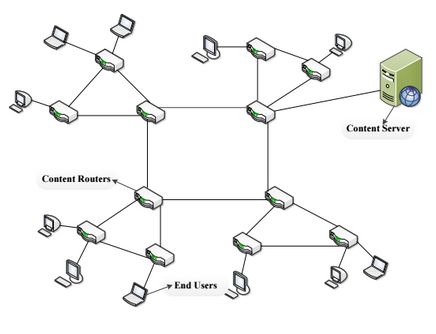
\includegraphics[width=10cm]{Imagenes/Paper1.1/Topologia_de_red}
	\caption{Sección de la topología de la red. Fuente: On Performance of Cache Policies in Named Data Networking \cite{ran2013performance}}
	\label{topologia_de_red}
\end{figure}

\subsubsection{Resultados}
A continuación se presentaran los resultados obtenidos respecto a las pruebas efectuadas a CCP en el simulador ndnSIM.

\begin{figure}[!htb]
	\centering
	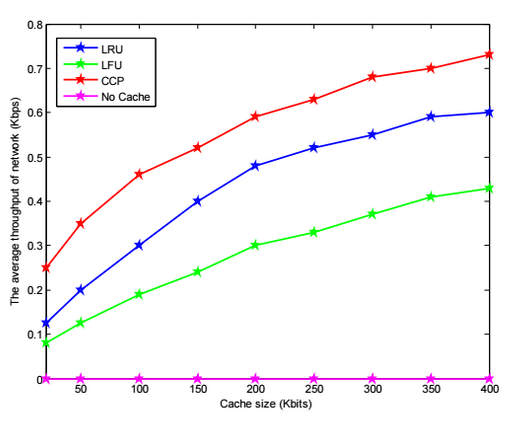
\includegraphics[width=8cm]{Imagenes/Paper1.1/Grafico_cache_hit_vs_size}\\
	\caption{Proporción de \textit{hit} en \textit{caché} VS Tamaño \textit{caché}. Fuente: On Performance of Cache Policies in Named Data Networking \cite{ran2013performance}}
	\label{hit_vs_size}
\end{figure}

\begin{figure}[!htb]
	\centering
	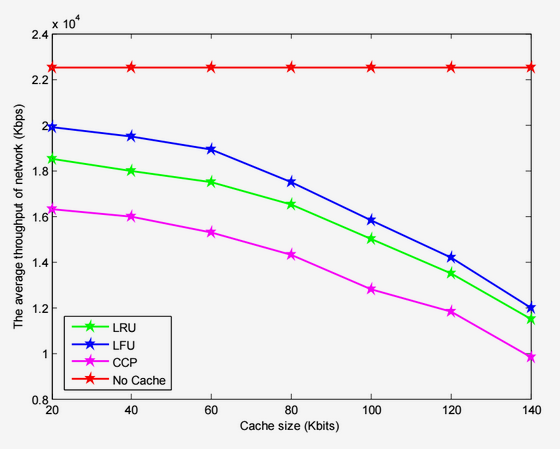
\includegraphics[width=10cm]{Imagenes/Paper1.1/Grafico_RendimientoRed_vs_cachesize}\\
	\caption{Rendimiento medio de la red VS Tamaño \textit{caché}. Fuente: On Performance of Cache Policies in Named Data Networking \cite{ran2013performance}}
	\label{RendimientoRed_vs_cssize}
\end{figure}

\begin{figure}[!htb]
	\centering
	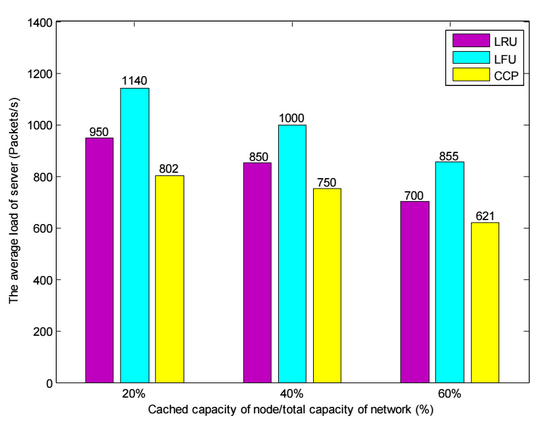
\includegraphics[width=10cm]{Imagenes/Paper1.1/Grafico_cargaservidor_vs_capacidadcache}\\
	\caption{ Carga media del servidor VS Capacidad \textit{caché}. Fuente: On Performance of Cache Policies in Named Data Networking \cite{ran2013performance}}
	\label{cargaServidor_vs_CapacidadCS}
\end{figure}

\clearpage

\subsection{Performance of probabilistic caching and cache replacement policies for content-centric networks \cite{tarnoi2014performance}.}

En este trabajo se habla principalmente entre la diferencia de lo que es un esquema de \textit{caché} y una política de reemplazo, entregando detalles de cada uno de estos. El trabajo \cite{tarnoi2014performance} tiene como objetivo el estudio del esquema de \textit{caché} probabilístico por medio de la simulación por computadora (ndnSIM) respecto a la utilización de diversas políticas de reemplazo de \textit{caché} (LRU, LFU y \textit{Randomly Replace}), esto debido a la simpleza del esquema de \textit{caché} probabilístico en comparación con otros esquemas \textit{caché} los cuales agregan una complejidad significativa y gastos generales en cuanto respecto a los sistema de almacenamiento en \textit{caché}. Basándose \cite{tarnoi2014performance} en que el comportamiento del esquema \textit{caché} probabilístico nunca han sido estudiada, y solo teniendo en cuenta el uso de la política de reemplazo LRU y de la cual no se definió un criterio que entregara un valor decente de la probabilidad de \textit{caché} así como su limitación practica.\\

Con respecto a lo definido en el trabajo \cite{tarnoi2014performance} se habla de dos tipos de esquemas de \textit{caché}. El primero denominado esquema de \textit{caché} universal(\textit{Always}) donde $p = 1$ y se caracteriza por el uso de una política de decisión de almacenamiento en \textit{caché} en cada uno de los \textit{router}(CR).Lo que si bien puede distribuir rápidamente el contenido en la red, se tiene evidencia de que este tipo de esquema puede poner replicas de los mismos objetos de contenido en múltiples \textit{routers} (CR),lo que degrada el rendimiento del \textit{caché} en la red provocando bajas tasas de \textit{hit's} en \textit{caché} en los \textit{routers} intermedios.\\

El segundo esquema denominado esquema de \textit{caché} probabilístico $prob(p)$ nombrado en \cite{psaras2014network}\cite{rossini2013evaluating} y \cite{cho2012wave}. Consiste en en que cada enrutador CCN almacena en \textit{caché} aleatoriamente un objeto de contenido que lo atraviese, basándose en una probabilidad de \textit{caché} definida como p, donde $0 < p < 1$. Este tipo de esquema solo ha sido probado solo con una política de reemplazo de \textit{caché} LRU con $p = 0,1$ siendo el valor más bajo de p que se ha usado[4]. Por lo que en este trabajo se propone reducir aun más el valor de p para:

1)Disminuir la probabilidad de \textit{caché} p en Prob (p) reduce la probabilidad de que múltiples \textit{routers} CCN en una ruta de entrega almacenen en \textit{caché} el mismo objeto de contenido en una entrega de contenido.
2) Disminuir la probabilidad de \textit{caché} p de Prob (p) resulta en una duración más larga del estado inicial de los sistemas de almacenamiento en \textit{caché}.\\

La puesta en marcha del trabajo descrito consta de la evaluación de los dos esquemas de \textit{caché}(universal, Prob(p)) cuando son puestos a trabajar con las políticas de reemplazo LRU, LFU y RR. Se utilizo ndnSIM el cual es un simulador basado en NS-3 modelando así el enrutamiento del intercambio de paquetes de interés y paquetes de datos los cuales poseen un tamaño fijo igual para todos.\\
Para la probabilidad de almacenamiento en \textit{caché} p se asignaron los siguiente valores (1, 0,7, 0,3 y 0,01). Ademas el CS de cada nodo comienza vació (arranque frio) y su tamaño varia entre el 1\% al 10\% de la población de contenido y se uso un algoritmo de Dijkstra para calcular el camino más corto (numero de saltos) para llegar al proveedor de contenido.\\

En cuanto a los solicitantes y proveedores de contenidos, el primero sigue una distribución Poisson con una media de 50 peticiones y el segunda consta de 1.000 objetos de contenidos diferentes. La simulación tuvo un tiempo de ejecución de 10.000 segundos y un calentamiento de 4.000 segundos.\\

La topología utilizada para representar la simulación fueron dos:

\begin{itemize}
	\item \textbf{Red en cascada}\\
	Red de longitud fija con cinco enrutadores Fig. \ref{Topologia_cascada}, de la cual se consideraron dos casos de estudios, con un solicitantes de contenidos y con múltiples solicitantes de contenido.
	\begin{figure}[!htb]
		\centering
		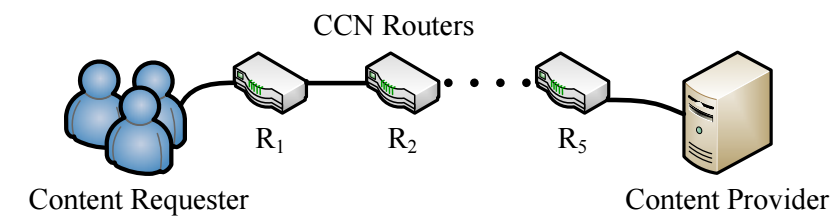
\includegraphics[width=10cm]{Imagenes/Topologia_cascada}\\
		\caption{Red cascada usada en la simulación. Fuente: Performance of probabilistic caching and cache replacement policies for content-centric networks \cite{tarnoi2014performance}}
		\label{Topologia_cascada}
	\end{figure}
	
	\item \textbf{SINET4}\\
	Topología híbrida de una red de malla y un numero de redes con topología estrella. Esta topología consta de ocho nodos centrales y 42 nodos de borde.
\end{itemize}

Las métricas a considerar para los resultados son los siguientes, carga del servidor, \textit{round-trip hop}, \textit{caché} \textit{hit rate}, comportamiento instantáneo.

\subsubsection{Resultados}

\subparagraph{Redes en Cascada}
Los resultados entregan que la carga del servidor disminuye como una función del tamaño CS para todos los casos. En el caso de Prob(p) + LRU reduce la carga de servidor a medida que p disminuye p, como lo fue con Prob(0,01) + LRU que logro un 20\% de mejora respecto a Always + LRU. Caso contrario es Prob(p) + LFU y Always + LFU, donde la carga del servidor aumenta a medida que se disminuye p, debido ha que los \textit{routers} con LFU pueden acumular objetos obsoletos. Por otro lado Prob(p) + RR no produce ningún cambio significativo en los resultados en términos de la reducción de carga del servidor, respecto a los valores entregado por p, siendo los resultados para Always + RR y Prob(p) + RR son casi idénticos.\\

En cuanto a los resultados obtenidos a la métrica de distancia de salto de ida y vuelta, entregando que Always + LRU es inferior al de Always + RR en el primer caso de estudios. Ya en el segundo Always + RR es idéntico. Por ultimo se analizo la tasa de \textit{hit} en \textit{caché}, de los cual se concluye que Always + LFU entrega las mejores tasas de éxito para todos los nodos. Seguido de Prob(0,01) + LRU y Always + LRU respectivamente. 

\subparagraph{SINET4}
Para la carga del servidor, los resultados entregados son similares a los entregados en la anterior topología. Ahora, en lo que respecta a la distancia de salto de ida y vuelta para diferentes esquemas de \textit{caché} y política, se  observar en los gráficos entregados que según el porcentaje de tamaño del \textit{caché} Always y  Prob(0.03, 0.07, 0.01)+ RR tiene el mejor resultado entregado, seguido de Always + LRU.\\

En cuanto al  porcentaje de \textit{hit} de los nodos, para el sector del núcleo de la topología, se obtuvo que Prob(0.01) + LRU tiene el mayor porcentaje de \textit{hit}, cercano al 40\%. Por otro lado el sector del borde de la topología entrega que Prob(0.01) + LRU entrega el mayor resultado con un 65\%, seguido de Always + LFU con un 63\%.\\

\pagebreak


\subsection{Cache Sharing Using Bloom Filters in Named Data Networking \cite{mun2017cache}}

Se define una paquete resumen (\textit{summary packet}) usando \textit{Bloom Filter} y un método para compartir el resumen. Esto cuando un paquete de datos es recibido, el \textit{routers} toma la decisión de si guardar o no el dato, dependiendo de el resultado de la consulta en \textit{caché} de los resúmenes de los \textit{routers} vecinos. Si alguno de los \textit{routers} vecinos tiene el dato, entonces el dato no tiene que ser necesariamente guardado. De otra manera, si un paquete de interés es recibido por un \textit{routers} entonces este mismo puede reenviarlos a sus \textit{routers} vecino analizando sus resúmenes. Todo esto con el fin de aumentar la diversidad de contenido en \textit{caché} en NDN. En este trabajo se utilizo una topología de 6 nodos Sprint PoP Fig. \ref{Topologia_Sprint_PoP} Mientras que los ajustes de los parámetros para la simulación se encuentran descritos en la Fig.\ref{Tabla_paremetros}

	\begin{figure}[!htb]
		\centering
		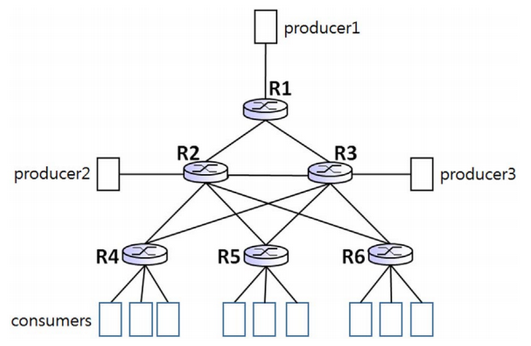
\includegraphics[width=10cm]{Imagenes/Topologia_Sprint_PoP}\\
		\caption{Topología 6-node Sprint PoP. Fuente: \cite{Spring:2002:MIT:964725.633039}}
		\label{Topologia_Sprint_PoP}
	\end{figure}
	
		\begin{figure}[!htb]
			\centering
			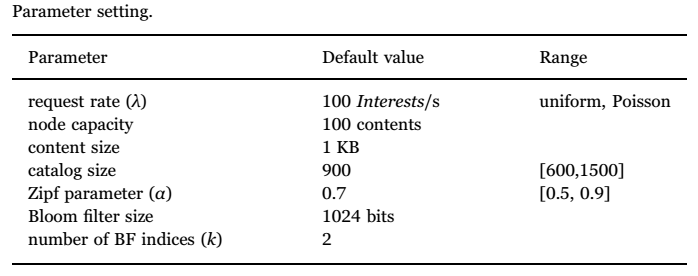
\includegraphics[width=10cm]{Imagenes/Tabla_parametros}\\
			\caption{Ajuste de parámetros. Fuente: Cache Sharing Using Bloom Filters in Named Data Networking \cite{mun2017cache}}
			\label{Tabla_paremetros}
		\end{figure}
	
Se aplican las políticas de reemplazo LRU y LFU correspondientes al simulador, siendo LRU-SS y LFU-SS las políticas con resumen compartido. Ademas se utilizo la política LCProb ya mencionada en \cite{ZHANG20133128} la cual deja copias de contenido en el camino de la ruta con una cierta probabilidad. El conjunto de métricas para la evaluación el rendimiento de los esquemas corresponden a: Éxito en \textit{caché} (\textit{caché hit}), diversidad de contenido y el tiempo de entrega del contenido.\\

Los resultados obtenidos por el trabajo se clasifican según el tipo de distribución utilizada (Uniforme y Poisson):

\paragraph{Cache Hit's (\%)}
En cuanto a la métrica de \textit{hit's} de \textit{caché} la política que alcanzo un mayor porcentaje fue la de LFU-SS de la distribución uniforme, la que tuvo un comienzo acierto del 65\% con 200 contenidos, para luego ir descendiendo hasta llegar a un 43\% con 500 contenidos. La que obtuvo peor resultado fue la política LRU de la distribución Poisson.

\paragraph{Diversidad de contenido(\%)}
Los mejores resultados los tuvo la política LRU-SS de la distribución Poisson, con un resultado que va entre un 60\% para luego aumentar a un 68\% aproximadamente en un intervalo de 200 a 500 contenidos respectivamente. El peor rendimiento lo tuvo la política LRU de la distribución Poisson.\\

\paragraph{Tiempo de entrega del contenido(ms)}
La política que entrego mejor resultado es la de LRU de la distribución uniforme con un tiempo mínimo de 7,6 para luego aumentar a 10,5, con 200 y 500 contenidos respectivamente. El peor resultado lo dio LFU-SS de la distribución Poisson, con una máxima de 9.5 aprox.\\

\paragraph{Parámetros Zipf ($\alpha$)}
También en este trabajo se obtuvieron análisis del parámetro $\alpha$ de zipf que van desde 0,5 a 0,9 y al igual que los resultados anteriores, están clasificados según el tipo de distribución utilizada. Los Resultados fueron los siguientes:

\begin{itemize}
	\item \textbf{Cache Hit's (\%):} 
	Si bien LFU-SS de la distribución uniforme con $\alpha = 0,5$ obtuvo el mejor resultado en la primera instancia con un total de 43\% aprox., a medida que $\alpha$ aumenta LFU-SS y LRU-SS de la misma distribución llegan al mismo resultado de 65\% de \textit{hit's}.
	\item \textbf{Diversidad de contenido(\%):}
	El mejor resultado lo tuvo sin duda la política LRU-SS de la distribución uniforme partiendo con un 66\% para luego seguir manteniéndose hasta llegar a un 65\%.
	\item \textbf{Tiempo de entrega del contenido(ms):}
	Respecto a esta métrica, el mejor resultado lo tiene la política LRU de la distribución uniforme partiendo con 10,3 ms aproximadamente llegando a un tiempo de 7,6 ms. La peor política es la de LFU-SS tanto en la distribución uniforme y Poisson.
\end{itemize}

\section{Arquitecturas de Caches}

\subsection{Two level caching technique for improving result ranking \cite{singh2011two}.}

En el siguiente trabajo \cite{singh2011two} se propone un esquema el cual reduce los requerimientos de entrada/salida y el computo, aumentando la escalabilidad de los motores de búsqueda web sin modificar el \textit{ranking} de este. Es una arquitectura de \textit{caché} que se compone de dos niveles que mezcla de forma paralela el \textit{caché} de listas invertidas y el \textit{caché} de resultados.\\

En el \textit{caché} de listas invertida se quiere evitar el acceso al disco el cual genera retraso, a través de la mantención en memoria de una lista la cual contiene documentos web's ligados a un término de la consulta. Por lo que al llegar una petición con un idéntico termino, esta tiene la posibilidad de ser respondida por la lista previamente almacenada. Además en este \textit{caché} se incluye una técnica para el almacenamiento de las listas invertidas, la cual consiste en ordenar la lista invertida respecto la  frecuencia con la que aparece el termino en cada documento, de modo que solo se usaran los termino que tengan alta frecuencia. Por eso es que la lista no se recorre completamente, además estas listas se dividen en bloques de documentos los que contienen los términos de la misma frecuencia.\\

Por otro lado el \textit{caché} de resultados, consiste en la utilización de una lista de documentos asociados a la consulta, en la cual para cada uno de estos documentos se guarda, el titulo, la URL y 250 caracteres.\\
\clearpage

El \textit{caché} propuesto en el trabajo \cite{singh2011two}(Fig. \ref{Esquemacache_2niveles}) combina lo mejor de los dos \textit{cachés} anteriormente mencionados, y cada vez que se lleva a cabo una petición se revisa si se encuentra en el \textit{caché} de resultado, si la petición es encontrada (\textit{hit}) entonces se responde inmediatamente y si no, entonces se revisa si se encuentra en el \textit{caché} de listas invertidas, por lo tanto si se genera \textit{hit} se mitiga el numero de acceso al disco pero si se genera \textit{miss} entonces se es necesario acceder a disco a encontrar la respuesta.

\begin{figure}[!htb]
	\centering
	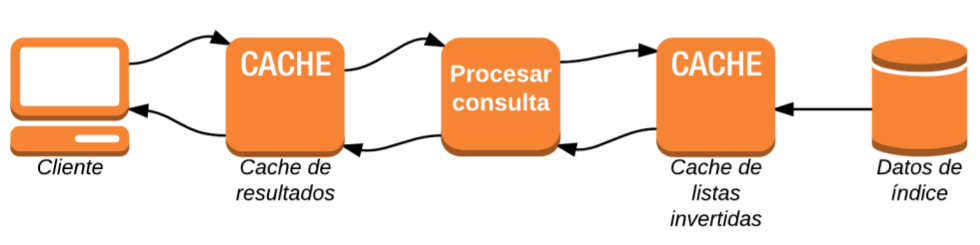
\includegraphics[width=10cm]{Imagenes/Paper2.1/EsquemaCache_2niveles}\\
	\caption{Esquema \textit{caché} de dos niveles. Fuente: Two level caching technique for improving result ranking \cite{singh2011two}}
	\label{Esquemaca
		che_2niveles}
\end{figure}
Como conclusión, los resultados obtenidos de los experimentos realizados en el motor de búsqueda "TodoBR" dan cuenta que el esquema de \textit{caché} utilizado es un 36\% mayor a que si solo se usara el \textit{caché} de resultado, y 52\% en comparación con el \textit{caché} de listas invertidas respecto al \textit{throughput}. 

\subsection{Time-based query classification and its application for page rank \cite{chen2011time}.}

Este trabajo consta de la clasificación de las paginas y consultas con el fin de mejorar el resultado de \textit{ranking}. En la Fig. \ref{clasificacion_consulta_tiempo} se puede observar como son clasificadas las consultas según el tipo que correspondan respecto a su temporalidad (permanentes, ráfaga, periódicas y ráfaga múltiple).

\begin{figure}[!htb]
	\centering
	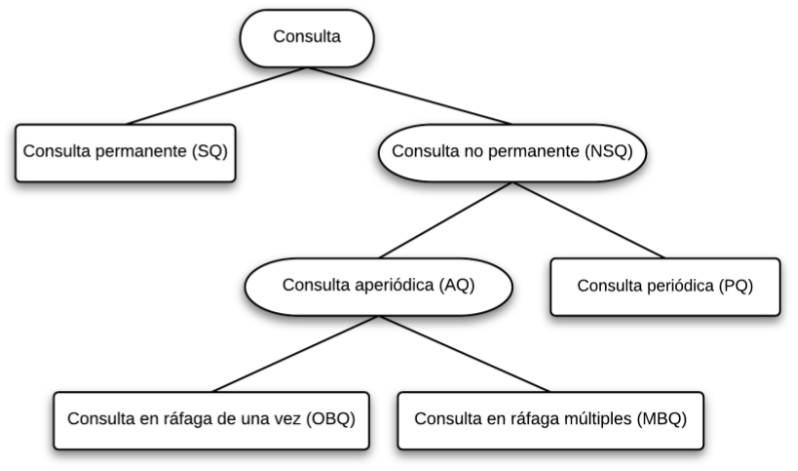
\includegraphics[width=8.5cm]{Imagenes/Clasificacion_consulta_tiempo}\\
	\caption{Clasificación de consultas basadas en el tiempo. Fuente: Time-based query classification and its application for page rank \cite{chen2011time}.}
	\label{clasificacion_consulta_tiempo}
\end{figure}

Para llevar a cabo lo anteriormente señalado. Primero se desarrolla un algoritmo que es el encargado de clasificar la categoría a la que corresponde una consulta según el registro de las peticiones pasadas. En segundo lugar se usa un modelo dinámico teórico el cual establece el \textit{rank} de las paginas respecto al tiempo de la publicación en la web y la información temporal contenida en la categoría de la consulta.\\

Entendido lo anterior, la clasificación se lleva a cabo de la siguiente manera. Cuando llega una consulta nueva el algoritmo desarrollado, clasifica la consulta según corresponda (permanente, periódica, ráfaga o ráfaga múltiple). Luego es utilizado el modelo dinámico propuesto (\textit{time-sensitive}), que entrega como salida el \textit{rank} de la pagina y la cual puede variar según la clasificación que fue designada la consulta entrante. Este método de \textit{ranking} usados, superan a los del método \textit{baseline ranking}.\\


\section{Organización del Caché}

\subsection{Políticas de desalojo}
Según lo leído en la literatura específicamente en los trabajos de \cite{wong2006web}\cite{podlipnig2003survey} etas políticas se pueden clasificar en:

\subsubsection{Basada en la frecuencia}
Son estrategias que tienen como base la utilización de la frecuencia (tamaño y/o costo) con la que es llamado un objeto, para decidir si reemplazar o no un objeto en \textit{caché}. Resultando así una mayor cantidad de \textit{hit} en \textit{caché}. Una de estas estrategias basadas en frecuencia es:
\begin{itemize}
	\item \textbf{\textit{Least Frequently Used} (LFU)}\\
	LFU Posee una complejidad algorítmica de $O(\log(n))$ y su función es la de eliminar la entrada menos frecuente referenciada. Pero LFU posee problemas, debido a que si un objeto posee una cantidad de frecuencia muy alta, y luego se convierte en impopular, entonces para que salga de \textit{caché} debe pasar un largo tiempo ha esto se le denomina corrupción de \textit{caché} \cite{wong2006web}.
\end{itemize}
\clearpage

\subsubsection{Basada en los reciente}
\begin{itemize}
	\item \textbf{\textit{Least Recententle Used} (LRU)}\\
	Una de las políticas de reemplazo más populares, todo gracias a su sencillez y muy bien catalogado rendimiento en diferentes escenarios \cite{wong2006web} y con una complejidad de  $O(1)$ . La política LFU desaloja la entrada menos referenciada recientemente en \textit{caché}. Cuando una cantidad grande de usuarios poseen un interés en común de objetos web, entonce se dice que existe una alta localidad temporal, escenario en donde la política LFU se destaca.
		
	\item \textbf{\textit{Probability Driven Cache} (PDC)\cite{lempel2003predictive}}\\
	Modelo probabilístico desarrollado para motores de búsqueda, debido ha que estos mismos guardan los resultados en memoria \textit{caché}. En \cite{lempel2003predictive} se explica que los motores de búsqueda entregan una enorme cantidad de paginas de resultados, de las cuales solo la primera es visitada por la mayoría de os usuarios. Por lo tanto almacenar el resto de paginas no es eficiente. Para mitigar esto, el modelo propuesto prioriza las paginas que están en \textit{caché} respecto al numero de usuarios que actualmente esta navegando las paginas que se dieron como resultados de la consulta.\\
	
	La política almacena las paginas de resultados que son visitadas actualmente respecto a la consulta y reemplaza o desaloja los resultados que no son relevantes o bien no poseen un flujo de visitas importante en aquel instante. Entregando como resultado un aumento del 50\% respecto a la política LRU.\\
	
\end{itemize}
\subsubsection{Basada en los frecuente/reciente}
\begin{itemize}
	\item \textbf{\textit{Hyper-G}}\\
	Política que combina lo mejor de tres políticas existentes (LRU, LFU, \textit{Size}), utilizando cada una de estas políticas en el orden respectivo, siempre y cuando se generen conflictos con objetos que cumplen el mismo criterio para el desalojo de este. La complejidad del la política corresponde ha $O(\log(n))$ y fue introducida primeramente en el trabajo de \cite{abrams1996removal}.
\end{itemize}
\clearpage

\subsubsection{Basada en tamaño del objeto}
\begin{itemize}
	\item \textbf{\textit{Size}}\\
	Su Complejidad es de $O(\log(n))$ y se caracteriza por el desalojo prioritario de entradas de mayor tamaño, por medio de colas de prioridad. En muchos casos el tamaño de los objetos web suelen ser fijos, por lo que en estos casos, se toma en cuenta una variable temporal la cual ayuda para el desalojo \cite{wong2006web}.
\end{itemize}

\subsubsection{Basada en funciones}
Tal como dice su nombre son estrategias las cuales se basan en la utilización de funciones, y parámetros tales como tiempo, tamaño, costo, latencia, frecuencia, entre otros. Para determinar si un objeto es desalojado o no, algunas de estas estrategias son:
\begin{itemize}
	\item \textbf{\textit{Least Unified Value}(LUV)}\\
	Política que unifica las ya conocidas políticas LRU y LFU. Por medio de la utilización de la formula 4.4 la que entrega un valor V(i) a cada documento , para esto esto la política utiliza la información de los objetos referenciados recientemente y la frecuencia de estos.
	
	\begin{equation}
	V(i) = W(i) * p(i)
	\end{equation}
	
	$W(i)$ corresponde al costo estimado de ir a buscar el objeto al servidor y $p(i)$ a la probabilidad de que un objeto \textit{i} sea referenciado en el futuro. Para calcular $W(i)$ se utiliza la función la descrita a continuación
	
	 \begin{equation}
	 W(i) = \frac{c_i}{s_i}
	 \end{equation}
	
	de la cual $c_i$ representa el costo y $s_i$ el tamaño del objeto. Por otro lado para calcular $p(i)$ se utiliza la siguiente función:
	
	\begin{equation}
		 p(i) = \displaystyle\sum_{k=1}^{f_i} F(t_c - t_k) 
	\end{equation}
	
	donde $t_c$ y $t_k$ son el tiempo actual y el tiempo en que se referencia el documento en un instante \textit{k} respectivamente. De 4.6 surge también 4.7 el cual entrega el valor de $\lambda$ y permite a LUV determinar medida que $\lambda$ es cercano a 1 entonces se da más énfasis a la información reciente, de lo contrario si $\lambda$ es cercano a 0 se enfatiza más la información de la frecuencia.
	
		\begin{equation}
		F(x) = \left(\frac{1}{2}\right)^{\lambda x}\textrm{, donde $0 \leq \lambda \leq 1$}
		\end{equation}
	
	LUV reemplaza el documento de menor valor, el que cambia solo cuando se accede a el. La complejidad de LUV es de $O(\log(n))$ y fue nombrado primeramente en el trabajo de \cite{bahn2002efficient}.
	
	\item \textbf{\textit{Hybrid}}\\
	Por otro lado se encuentra la política de desalojo \textit{Hybrid} la cual reemplaza los documentos respecto al tiempo de conexión al servidor para acceder a el ($c_s$), el ancho de banda con el servidor ($b_s$), el numero de veces referenciado el documento en \textit{caché} ($f_i$) y el tamaño del documento ($s_i$). Para determinar que documento ha reemplazar se utiliza la siguiente función:

	\begin{equation}
	v_i = \left(c_s + \frac{W_b}{b_s}\right) * \frac{(f_i)^{W_n}}{s_i}
	\end{equation}
	
	donde ademas de las variables mencionadas anteriormente se agregan $W_n$ y $W_b$ que son constantes que determinan la importancia relativa de las variables $f_i$ y $b_s$ respectivamente.\\
	
	Según lo descrito en 4.8 la política de desalojo \textit{Hybrid} tiene menores probabilidades de reemplazar los documentos que poseen un ancho de banda de conexión bajo, el tamaño del documento es pequeño, es referenciado varias veces y/o el tiempo para conectarse al servidor que lo contiene es alto. La complejidad de la política es de $O(\log(n))$.

\end{itemize}

\subsubsection{Asignación al azar}

\subparagraph{LRU-S:}
Política nombrada en el trabajo de , y corresponde a la utilización de la densidad normalizada de un objeto \textit{i} correspondiente ha $d_i = \frac{S_min}{S_i}$, donde $S_min$ corresponde al tamaño mínimo de los N objetos almacenados en \textit{caché}. Por lo tanto LRU-S varia de lugar los objetos $i$ según el valor entregado por $d_i$. La complejidad de LRU-S es de $O(1)$.



\subsection{Políticas de admisión}

\subsubsection{Admission Policies for Caches of Search Engine Results \cite{baeza2007admission}.}

Política de admisión propuesta en el trabajo de \cite{baeza2007admission} la que busca clasificar si una consulta es frecuente o infrecuente antes de que esta entre en \textit{caché} por medio de un estimador. El diseño de la política, consiste en dividir el \textit{caché} en dos. La primera sección están las consultas que la política predice podrían tener \textit{hitś}, esta sección es denominada \textit{caché} controlado (CC). La segunda sección es denominada \textit{caché} no controlado (UC) y es donde se envían las consultas que no fueron aceptadas por la política. 

\begin{figure}[!htb]
	\centering
	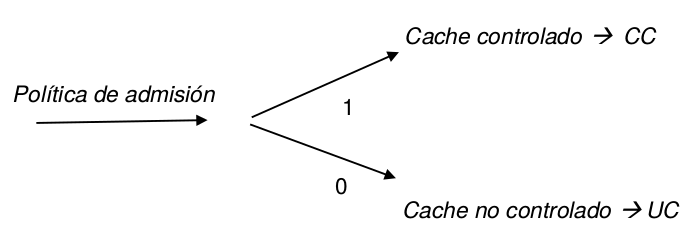
\includegraphics[width=12cm]{Imagenes/PoliticaAdmi_cache_CC_UC}\\
	\caption{Clasificación de consultas según política. Fuente: Admission Policies for Caches of Search Engine Results \cite{baeza2007admission}.}
	\label{clasificacion_consulta_cc_uc}
\end{figure}

Para lograr entrar al \textit{caché} controlado se toma en cuenta la política de admisión basada en umbral K. Existen dos, el primero es una umbral estático y respecto al numero de palabras, y el segundo corresponde a un umbral dinámico el cual toma en cuenta lo caracteres no alfanuméricos en la consulta, de modo que una consulta con varios caracteres alfanuméricos no llegara a ser popular. Los resultados demuestran una mejora del 21\% respecto ha \textit{Least Recentently Used} (LRU) y un 4\% en relación a \textit{Static Dynamic Cache} (SDC) de un total de 100.000 consultas.\\

\clearpage


\subsubsection{TinyLFU: A highly efficient cache admission policy}
Política propuesta en \cite{einziger2014tinylfu}, la cual busca aumentar la eficacia del \textit{caché}. Esta política se basa en la frecuencia aproximada y consiste en en tener almacenadas las estadísticas de las frecuencia de los ítems, con el objetivo de decidir si permitir la nueva entrada, tomando en cuenta al candidato a desalojar en \textit{caché} la cual se le denomina ``víctima".\\

\begin{figure}[!htb]
	\centering
	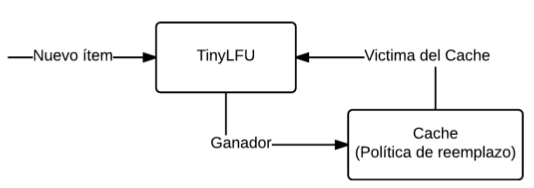
\includegraphics[width=12cm]{Imagenes/Politica_TinyLFU}\\
	\caption{Arquitectura TinyLFU. Fuente:.\cite{einziger2014tinylfu}}
	\label{clasificacion_consulta_cc_uc}
\end{figure}

Debido ha que almacenar la estadística de las frecuencia de los ítems tiene un gran costo, es necesario llevar a cabo técnicas de recuento aproximado para las frecuencias con el fin de disminuir el consumo de memoria. Una técnica para esto es la denominada \textit{Counting Bloom Filter} (CBF).\\

El \textit{Bloom Filter} es una estructura con datos probabilísticos lo cual permite saber de manera eficiente si un dato existe o no en un conjunto. Por lo que el \textit{Counting Bloom Filter} es un tipo de \textit{Bloom Filter}.
Para cada política utilizada (LRU, Random, TLRU (LRU incorpora TinyLFU), TRandom (Random incorpora TinyLFU), TLFU (LFU incorpora TinyLFU), W-TinyLFU, LIRS y ARC). Las conclusiones obtenidos por esta demuestran que la tasa de \textit{hit} en las que utilizan esta política de admisión es mejor en comparación con las otras, destacándose entre estas TLRU y W-TinyLFU.\\


\chapter{Propuesta}

Para lo anterior, la solución propuesta en este trabajo consiste en desarrollar una arquitectura de caché para los nodos de una red NDN, tomando en cuenta el comportamiento dinámico de los usuarios. Para ello se utilizara el simulador ndnSIM el que  ayudara a recrear una red basada en contenidos y obtener los resultados de la arquitectura caché propuesta.

\section{Escenario}

\subsection{Topologia y enlaces}

El conjunto de nodos interconectados entre si o dicho de otra manera la topologia utilizada para llevar a cabo este trabajo, es descrita como una matriz de tres por tres, la cual se encuentra dentro del la categoría de topologia de árbol. El enlace entre los nodos sigue un protocolo PPP (Point-to-Point Protocol). La representación gráfica de la topologia se puede apreciar en la Fig. \ref{topologia_3x3_plugin}
                                                                                                                                                                                                                   
\begin{figure}[!htb]                                                                                  
	\centering                                                        
	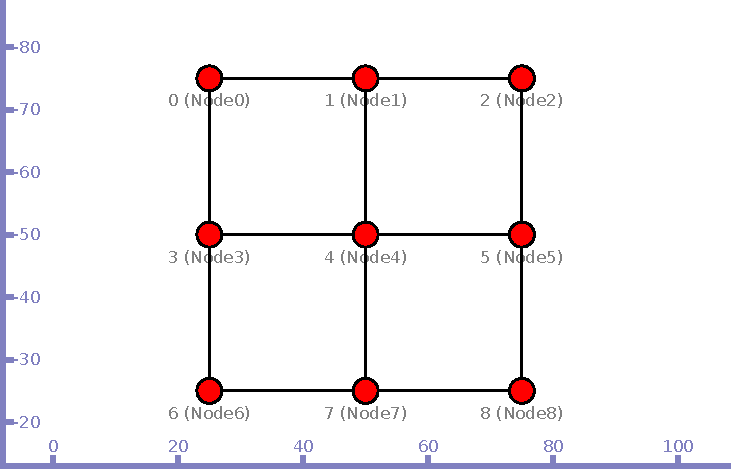
\includegraphics[width=8cm]{Imagenes/Matriz3x3.pdf}\\                                                             
	\caption{Topologia utilizada. Fuente: Elaboración propia}                                                                                                                                                         
	\label{topologia_3x3_plugin}
\end{figure}

\pagebreak

A continuación, en la Fig, se puede apreciar parte del código principal (main) en el cual se realiza la lectura de un archivo de texto, que contiene la estructura y los datos necesarios para crear la topologia usada en la simulación. Esto gracias a la clase 'AnnotatedTopologyReader'.

\begin{lstlisting}[language=cpp,caption={Codigo fuente: main},label={codigo_topologia}]
#include "ns3/core-module.h"
#include "ns3/network-module.h"
#include "ns3/ndnSIM-module.h"

namespace ns3 {

int
main(int argc, char* argv[]) // main
{
CommandLine cmd;
cmd.Parse(argc, argv);

AnnotatedTopologyReader topologyReader("", 25); 
topologyReader.SetFileName("extensions/topo-grid-3x3.txt"); // Se llama al archivo 
topologyReader.Read(); // Lecura del archivo con la topologia.
\end{lstlisting}

\pagebreak
Por otro lado en la Fig. se encuentra un fragmento del archivo de texto leído 'topo-grid-3x3-.txt' en donde se pueden configurar la estructura y los parámetros para el trafico de datos.

\begin{lstlisting}[frame=single]
...
# node  comment     yPos    xPos
Node0   NA          3       1
Node1   NA          3       2
Node2   NA          3       3
Node3   NA          2       1
Node4   NA          2       2
Node5   NA          2       3
Node6   NA          1       1
Node7   NA          1       2
Node8   NA          1       3
...

# srcNode    dstNode    bandwidth   metric    delay queue
Node0       Node1       1Mbps       1       10ms    10
Node0       Node3       1Mbps       1       10ms    10
Node1       Node2       1Mbps       1       10ms    10
Node1       Node4       1Mbps       1       10ms    10
Node2       Node5       1Mbps       1       10ms    10
Node3       Node4       1Mbps       1       10ms    10
Node3       Node6       1Mbps       1       10ms    10
Node4       Node5       1Mbps       1       10ms    10
Node4       Node7       1Mbps       1       10ms    10
Node5       Node8       1Mbps       1       10ms    10
Node6       Node7       1Mbps       1       10ms    10
Node7       Node8       1Mbps       1       10ms    10
\end{lstlisting}

En donde en la primera tabla donde se define los \textit{routers} ubicándolos en un plano cartesiano (X,Y) dentro del simulador y una segunda tabla en la que se definen los enlaces y sus variables tales como el nodo salida(srcNode), nodo destino(dstNode), ancho de banda(bandwidth), métrica de enrutamiento(metric), retraso(delay) y cola(queue) la que ajusta el máximo de transmisión de paquetes en el enlace(\textit{link}).

\pagebreak

\subsection{Arquitectura del caché}


\begin{lstlisting}[language=cpp,caption={Caption}]
NodeContainer nodo1, nodo2, nodo3, nodo4, nodo5, nodo6 ,nodo7, consumerNodes;

// Se instancia la variable ndnHelper
ndn::StackHelper ndnHelper;

ndnHelper.SetOldContentStore("ns3::ndn::cs::Double", "MaxSize", "10000");

nodo1.Add(Names::Find<Node>("Node1"));// Se busca el nodo segun nombre
ndnHelper.Install(nodo1); // Se instala la politica de reemplazo en el nodo 1 (ROUTER)
.
.
.
ndnHelper.SetOldContentStore("ns3::ndn::cs::Nocache"); // Se define la politica de NO CACHE

consumerNodes.Add(Names::Find<Node>("Node0")); // Se busca el nodo segun nombre
Ptr<Node> producer = Names::Find<Node>("Node8");// Se busca el nodo segun nombre

ndnHelper.Install(consumerNodes); // Se instala la politica de reemplazo en el nodo CONSUMIDOR
ndnHelper.Install(producer); // Se instala la politica de reemplazo en el nodo PRODUCTOR
\end{lstlisting}


\subsection{Consultas}
\subsubsection{Consumidor}

\begin{lstlisting}[language=cpp,caption={Caption}]
  std::string prefix = "/prefix";
  
  ndn::AppHelper consumerHelper("ns3::ndn::ConsumerCbr"); // Se crea la instancia
  consumerHelper.SetPrefix(prefix);       // Seteo del prefijo
  consumerHelper.SetAttribute("Frequency", StringValue("1")); // Seteo de la frecuencia en que enviara 
  // los intereses (1 por segundo).
  consumerHelper.Install(consumerNodes); // Se installa la aplicacion en uno o mas nodos.
\end{lstlisting}


\subsubsection{Productor}
\begin{lstlisting}[language=cpp,caption={Caption}]
ndn::AppHelper producerHelper("ns3::ndn::Producer"); // Se crea la instancia
producerHelper.SetPrefix(prefix); //Seteo del prefijo
producerHelper.SetAttribute("PayloadSize", StringValue("1024")); //
producerHelper.Install(producer); // Se instala la aplicacion en una o mas nodos.
\end{lstlisting}

\section{Arquitectura cache}
\subsection{Instalación}


\chapter{Enfoques metodológico}

\chapter{Pruebas y resultados}

\chapter{Conclusiones}
\section{Trabajo Futuro}


%*******************************************************
%next line adds the Bibliography to the contents page
\addcontentsline{toc}{chapter}{Bibliografia}
%uncomment next line to change bibliography name to references
%\renewcommand{\bibname}{References}
\bibliography{refs}        %use a bibtex bibliography file refs.bib
\bibliographystyle{plain}  %use the plain bibliography style

\end{document}

